%%%%%%%%%%%%%%%%%%%%%%%%%%%%%%%%%%%%%%%%

% PDF compatibility code. 



\makeatletter
\newif\ifpdflatex@
\ifx\pdftexversion\@undefined
\pdflatex@false
%\message{Not using pdf}
\else
\pdflatex@true
%\message{Using pdf}
\fi

\newcommand{\latexpdf}[2]{
  \ifpdflatex@ #1
  \else #2
  \fi
}

\newcommand{\latexorpdf}[2]{
  \ifpdflatex@ #2
  \else #1
  \fi
}

#ifdef A4Format
\newcommand{\pformat}{a4paper}
#endif A4Format
#ifdef LetterFormat
\newcommand{\pformat}{letterpaper}
#endif LetterFormat

\makeatother

%%%%%%%%%%%%%%%%%%%%%%%%%%%%%%%%%%%%%%%%

\latexorpdf{
\documentclass[\pformat,12pt]{article}
}{
% pdftex option is used by graphic[sx],hyperref,toolbox.sty
\documentclass[\pformat,pdftex,12pt]{article}
}

\usepackage[dvipdfmx]{graphicx, color}
\usepackage[dvipdfm,bookmarks=true,bookmarksnumbered=true,colorlinks,plainpages=true]{hyperref}

\usepackage{toolbox}
\usepackage{makeidx}
\usepackage{here}
\usepackage{verbatimfiles}
\usepackage{ifthen}
\usepackage{longtable}
\usepackage{array}

% Ueki change start
%#ifdef JPN
%\AtBeginDvi{\special{pdf:tounicode 90ms-RKSJ-UCS2}}
%#endif JPN

\usepackage{cite}

\def\seename{$\Rightarrow$}
% Ueki change end

% Ueki delete start
%\latexorpdf{
%\usepackage[plainpages=true,colorlinks,linkcolor=black,citecolor=black,pagecolor=black, urlcolor=black]{hyperref}
%}{
%\usepackage[plainpages=true,colorlinks]{hyperref}
%}
% Ueki delete end

\usepackage{color}
\newcommand{\vdmsl}{VDM-SL }
\newcommand{\vdmpp}{VDM++ }

\makeindex


% Following command used to preserve backslash in tabular environments
\newcommand{\pbs}[1]{\let\temp=\\#1\let\\=\temp}

\newenvironment{interfacetable}{%
  \begin{longtable}{|>{\pbs\raggedright\ttfamily}p{6.6cm}%
                    |>{\pbs\raggedright}p{6.6cm}|} \hline
  \textrm{\bfseries Name} &  \textbf{Description} \\ \hline
  \endhead
  }{\end{longtable}}

\newcommand{\APIError}{\hyperlink{exception.APIError}{raises APIError}}
\newcommand{\VDMError}{\hyperlink{exception.VDMError}{raises VDMError}}
\newcommand{\Generic}{\hyperlink{interface.Generic}{Generic}}
\newcommand{\VDMGeneric}{\hyperlink{interface.Generic}{VDMGeneric}}
\newcommand{\ModuleName}{\hyperlink{type.ModuleName}{ModuleName}}
\newcommand{\ModuleList}{\hyperlink{type.ModuleList}{ModuleList}}
\newcommand{\ClassName}{\hyperlink{type.ClassName}{ClassName}}
\newcommand{\ClassList}{\hyperlink{type.ClassList}{ClassList}}
\newcommand{\FileName}{\hyperlink{type.FileName}{FileName}}
\newcommand{\FileList}{\hyperlink{type.FileList}{FileList}}
\newcommand{\ToolType}{\hyperlink{type.ToolType}{ToolType}}
\newcommand{\ErrorStruct}{\hyperlink{struct.Error}{Error}}
\newcommand{\ModuleStatus}{\hyperlink{struct.ModuleStatus}{ModuleStatus}}
\newcommand{\VDMApplication}{\hyperlink{interface.VDMApplication}{VDMApplication}}
\newcommand{\VDMCodeGenerator}{\hyperlink{interface.VDMCodeGenerator}{VDMCodeGenerator}}
\newcommand{\VDMErrors}{\hyperlink{interface.VDMErrors}{VDMErrors}}
\newcommand{\VDMInterpreter}{\hyperlink{interface.VDMInterpreter}{VDMInterpreter}}
\newcommand{\VDMModuleRepos}{\hyperlink{interface.VDMModuleRepos}{VDMModuleRepos}}
\newcommand{\VDMFactory}{\hyperlink{interface.VDMFactory}{VDMFactory}}
\newcommand{\VDMParser}{\hyperlink{interface.VDMParser}{VDMParser}}
\newcommand{\VDMPrettyPrinter}{\hyperlink{interface.VDMPrettyPrinter}{VDMPrettyPrinter}}
\newcommand{\VDMProject}{\hyperlink{interface.VDMProject}{VDMProject}}
\newcommand{\VDMTypeChecker}{\hyperlink{interface.VDMTypeChecker}{VDMTypeChecker}}
\newcommand{\ClientID}{\hyperlink{type.ClientID}{ClientID}}
\newcommand{\bytes}{\hyperlink{type.bytes}{bytes}}
\newcommand{\VDMBool}{\hyperlink{interface.VDMBool}{VDMBool}}
\newcommand{\VDMChar}{\hyperlink{interface.VDMChar}{VDMChar}}
\newcommand{\VDMNumeric}{\hyperlink{interface.VDMNumeric}{VDMNumeric}}
\newcommand{\VDMQuote}{\hyperlink{interface.VDMQuote}{VDMQuote}}
\newcommand{\VDMText}{\hyperlink{interface.VDMText}{VDMText}}
\newcommand{\VDMToken}{\hyperlink{interface.VDMToken}{VDMToken}}
\newcommand{\VDMNil}{\hyperlink{interface.VDMNil}{VDMNil}}
\newcommand{\VDMMap}{\hyperlink{interface.VDMMap}{VDMMap}}
\newcommand{\Map}{\hyperlink{interface.VDMMap}{Map}}
\newcommand{\VDMRecord}{\hyperlink{interface.VDMRecord}{VDMRecord}}
\newcommand{\Record}{\hyperlink{interface.VDMRecord}{Record}}
\newcommand{\VDMSequence}{\hyperlink{interface.VDMSequence}{VDMSequence}}
\newcommand{\Sequence}{\hyperlink{interface.VDMSequence}{Sequence}}
\newcommand{\VDMSet}{\hyperlink{interface.VDMSet}{VDMSet}}
\newcommand{\Set}{\hyperlink{interface.VDMSet}{Set}}
\newcommand{\VDMTuple}{\hyperlink{interface.VDMTuple}{VDMTuple}}
\newcommand{\Tuple}{\hyperlink{interface.VDMTuple}{Tuple}}
  
% Following command used to put notes in drafts to remind author of
% incomplete parts
\newcommand{\note}[1]{\colorbox{red}{#1}}

\makeatletter
% ------------- TOC manipulation ------------
\def\docglbldepth{1}
%\setcounter{secnumdepth}{\docglbldepth}
%\setcounter{tocdepth}{\docglbldepth}
\def\@pnumwidth{3.0em}
% more space for for >10 subsections
%\def\l@section{\@dottedtocline{1}{1.5em}{3.1em}}
\def\l@subsection{\@dottedtocline{2}{1.5em}{2.8em}}
%\def\l@subsubsection{\@dottedtocline{3}{4.3em}{3.6em}}
%\def\l@paragraph{\@dottedtocline{4}{7.9em}{4.1em}}
%\def\l@subparagraph{\@dottedtocline{5}{10em}{5em}}
\makeatother

\makeindex


\begin{document}

\vdmtoolsmanualcsk{The VDM Toolbox API}
       {VDM-SL v9.0.6 and VDM++ v9.0.6}
       {2016}
       {VDM-SL/VDM++}
       {1.0}

\renewcommand{\thepage}{\roman{page}}

%\tableofcontents
\label{endtofc}
\ifthenelse{\isodd{\pageref{endtofc}}}{\mbox{}\newpage}{}
\newpage 
\renewcommand{\thepage}{\arabic{page}}
\setcounter{page}{1}


\section{Introduction}
This document describes how to use the CORBA-based API of the VDM Toolbox. 

The VDM Toolbox API allows you to write programs (clients) that access
and modify certain properties of a running instance of a VDM
Toolbox (graphical or command line). The
VDM Toolbox can be accessed by several CORBA clients at the same time.
These clients can - through the API - access and configure the
project, parse and type check individual files, evaluate expressions
through the interpreter, etc. The client processes and the VDM Toolbox
are separate processes that may run on different machines, possibly
running on different operating systems, on the network. As a
consequence, a VDM Toolbox being used as server by any client process
is also available to the user through its user interface.

The API is based on CORBA (see \cite{OMG&96}). For this reason the API is
accessible from any language for which there exists a CORBA
2.0 compliant implementation. For example you could easily write your client in
either C++ or Java, since several (free) CORBA implementations are
available for these languages. Throughout Section~\ref{Toolboxapi}
small pieces of example code written in C++ are provided. In
sections~\ref{writingacppclient} and \ref{writingajavaclient} however,
we will describe how to write a complete client in C++ and Java
respectively. 

This document and the API it describes apply to both the VDM-SL and
VDM++ version of the Toolbox. The API only differentiates between
VDM-SL and VDM++ in a few cases, and they are explicitly stated in the
definition of the API. In general, when we use the term ``module" in
this manual and in the definition of the API, we refer to either a
module in VDM-SL or a class in VDM++.   

\newpage
\section{CORBA - The Basics}

The main idea in CORBA is {\em distribution of objects}. A client
process can create, access and possibly modify the state of objects
handled by and physically contained in a separate server process
located locally or remotely on the network. The client has ``a
handle'' to the object contained in the server and it uses this handle
to make method calls, as if the distributed object is located in the
address space of the client. The CORBA standard specifies how a handle
to a distributed object can be acquired as well as how methods are
invoked, and values are passed between different objects. 

Since CORBA is only a standard for object distribution, an
implementation of CORBA (a so-called {\em ORB}) is necessary to write
CORBA servers and clients. Currently CORBA implementations are
available for a multitude of different platforms and languages.  

\subsection{IDL}

The objects exposed by a CORBA enabled server are described using the
Interface Definition Language (IDL). IDL is an object-oriented
language for describing interfaces in an implementation language and
in a platform neutral way. Vendors that provide tools with a CORBA
interface make the interface known to clients by distributing the IDL
description with the tool. The syntax of IDL is described in
\cite{OMG&96}. 

When implementing a client, the IDL description is mapped to the
preferred implementation language using an IDL compiler (comes with
the chosen CORBA implementation). The code generated from the IDL
description is compiled and linked with the client executable making
it capable of using the CORBA interface of the server. 

\newpage
\section{The VDM Toolbox API} 
\label{Toolboxapi}

The CORBA interface of the VDM Toolbox is described in the two IDL
files {\tt corba\_api.idl} and {\tt metaiv\_idl.idl}, that are also
distributed with the VDM Toolbox. The first file describes the actual
interface of the VDM Toolbox whereas the second file describes the
interface of different VDM values that can be passed between a client
and the VDM Toolbox. In the following both files will be described in
detail, and in Section~\ref{refguide} a reference manual for these 
interfaces is provided. 

\subsection{IDL Description of The Tool API}
\label{idldescriptiontool}

The API of the VDM Toolbox consists of a number of different objects
(interfaces in IDL) accessible from a client process. The object {\tt
  \VDMApplication}, from which all other aspects of the API are
available, is the main entry point. This object is the client's handle
to the VDM Toolbox, and must consequently be constructed prior to
using any other functionality of the API. In
section~\ref{writingacppclient} and Section~\ref{writingajavaclient}
we will describe how to acquire this handle to the VDM Toolbox in C++ 
and Java respectively.

\begin{figure}[tbh]
\begin{center}
\mbox{}
\resizebox{5cm}{!}{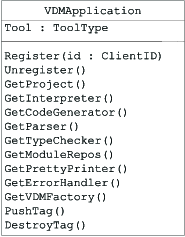
\includegraphics{VDMApplication.png}}
\caption{The {\tt VDMApplication} interface.}\label{fig:VDMApplication}
\end{center}
\end{figure}

%\begin{figure}[tbh]
%\begin{center}
%\begin{tabular}{|l|}
%\hline
%{\tt ToolboxAPI::VDMApplication } \\
%\hline
%{\tt Tool: ToolType } \\
%\hline
%{\tt Register () } \\
%{\tt Unregister(in VDM::ClientID id) } \\
%{\tt GetProject() }\\
%{\tt GetInterpreter() }\\
%{\tt GetCodeGenerator() }\\
%{\tt GetParser() }\\
%{\tt GetTypeChecker() }\\
%{\tt  GetPrettyPrinter() }\\
%{\tt GetErrorHandler() }\\
%{\tt GetModuleRepos() }\\
%{\tt GetVDMFactory() }\\
%{\tt PushTag(in VDM::ClientID id) }\\
%{\tt DestroyTag(in VDM::ClientID id) }\\
%\hline
%\end{tabular}
%\caption{The {\tt VDMApplication} interface.}\label{fig:VDMApplication}
%\end{center}
%\end{figure}

The {\tt \VDMApplication} interface is shown in
Figure~\ref{fig:VDMApplication}.  The methods {\tt Register} and {\tt
  Unregister} are used by a client to register and unregister its
process at the server.  Moreover, the {\tt \VDMApplication} interface
consists of a number of methods returning other interfaces. For
instance, if you wish to configure the current project of the VDM
Toolbox, use {\tt GetProject} to get a handle to the project
interface, that is, a handle to the {\tt \VDMProject} interface
described below. Additionally the {\tt Tool} attribute of the
interface can be used to decide the type of tool used as server, i.e.\
whether the client is connected to a VDM-SL or a VDM++ Toolbox.  For
detailed information on how to read and modify the value of attributes
see Sections~\ref{writingacppclient} and \ref{writingajavaclient}.
\subsubsection{VDMProject}

\begin{figure}[tbh]
\begin{center}
\mbox{}
\resizebox{7.5cm}{!}{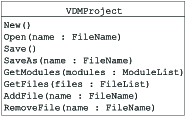
\includegraphics{VDMProject.png}}
\caption{The {\tt VDMProject} interface.}\label{fig:VDMProject}
\end{center}
\end{figure}

%\begin{figure}[tbh]
%\begin{center}
%\begin{tabular}{|l|}
%\hline
%{\tt ToolboxAPI::VDMProject } \\
%\hline
%{\tt New() } \\
%{\tt Open(in FileName name) } \\
%{\tt Save() } \\
%{\tt SaveAs(in FileName name) } \\
%{\tt GetModules(out ModuleList modules)} \\
%{\tt GetFiles(out FileList files)} \\
%{\tt AddFile(in FileName name)} \\
%{\tt RemoveFile(in FileName name)} \\
%\hline
%\end{tabular}
%\caption{The {\tt VDMProject} interface.}\label{fig:VDMProject}
%\end{center}
%\end{figure}



The {\tt \VDMProject} interface is shown in
Figure~\ref{fig:VDMProject}.  Using this interface it is possible to
access and modify the current project of the VDM Toolbox. 
{\tt GetFiles} and {\tt GetModules} return (through a parameter) a
sequence of file names and module names in the current project. {\tt
  AddFile} and {\tt RemoveFile} are used to configure the project.

\subsubsection{VDMModuleRepos}

The {\tt \VDMModuleRepos} interface is shown in
Figure~\ref{fig:VDMModuleRepos}.

\begin{figure}[tbh]
\begin{center}
\mbox{}
\resizebox{15cm}{!}{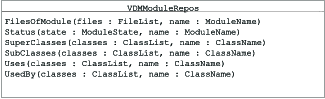
\includegraphics{VDMModuleRepos.png}}
\caption{The {\tt VDMModuleRepos} interface.}\label{fig:VDMModuleRepos}
\end{center}
\end{figure}

%\begin{figure}[tbh]
%\begin{center}
%\begin{tabular}{|l|}
%\hline
%{\tt ToolboxAPI::VDMModuleRepos } \\
%\hline
%{\tt FilesOfModule(out FileList files, in ModuleName name) } \\
%{\tt Status(out ModuleStatus state, in ModuleName name) } \\
%{\tt SuperClasses(out ClassList classes, in ClassName name) } \\
%{\tt SubClasses(out ClassList classes, in ClassName name) } \\
%{\tt UsesOf(out ClassList classes, in ClassName name) } \\
%{\tt UsedBy(out ClassList classes, in ClassName name) } \\
%\hline
%\end{tabular}
%\caption{The {\tt VDMModuleRepos} interface.}\label{fig:VDMModuleRepos}
%\end{center}
%\end{figure}

The interface {\tt \VDMModuleRepos} is used to acquire additional
information on a given module or class. {\tt FilesOfModule} returns
the files of a particular module, while {\tt Status} retrieves the
current status, as indicated by the S, T, C, and P indicators in the
user interface, of a given module. The four remaining methods are only
available from the VDM++ Toolbox. They are used to query the
inheritance and association relationships of a class. Use these
methods to find the super or sub classes of a class as well as to find
out how classes reference each other.  

Notice that, since this IDL description is common to both the VDM++
and VDM-SL Toolbox, whenever we use {\em \ModuleName} or {\em \ModuleList} in the
definitions this applies to both modules (from VDM-SL) and classes
(from VDM++). However if {\em \ClassName} or {\em \ClassList} is explicitly used,
application is restricted to VDM++ only.

\subsubsection{VDMParser}


\begin{figure}[tbh]
\begin{center}
\mbox{}
\resizebox{7.5cm}{!}{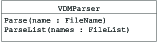
\includegraphics{VDMParser.png}}
\caption{The {\tt VDMParser} interface.}\label{fig:VDMParser}
\end{center}
\end{figure}

%\begin{figure}[tbh]
%\begin{center}
%\begin{tabular}{|l|}
%\hline
%{\tt ToolboxAPI::VDMParser } \\
%\hline
%{\tt Parse(in FileName name) } \\
%{\tt ParseList(in FileList names) } \\
%\hline
%\end{tabular}
%\caption{The {\tt VDMParser} interface.}\label{fig:VDMParser}
%\end{center}
%\end{figure}

The {\tt \VDMParser} interface is shown in Figure~\ref{fig:VDMParser}.
The interface can be used to have the VDM Toolbox parse either a
single file or a list of files. In the latter case the file list will
normally have been acquired by a call to 
\texttt{\hyperlink{method.VDMProject::GetFiles}{VDMProject::GetFiles}},
instead of manually constructing the list.

If errors are encountered while parsing the file(s) the {\tt
  \VDMErrors} interface (described in Section~\ref{VDMErrors}) can
subsequently be queried to gain detailed information describing the
errors detected. 

The structure of the interfaces for the type checker, code generator
and pretty printer ({\tt \VDMCodeGenerator}, {\tt \VDMTypeChecker} and
{\tt \VDMPrettyPrinter}) are very similar to {\tt \VDMParser}, with the
only difference that these interfaces have a number of different
attributes that can be read and modified from the client. The setting
of such attributes control the functionality of the particular
interface. These three interfaces will not be described in detail
here, and we refer to the IDL description in Section~\ref{refguide} for
further details and descriptions of the individual attributes.

\subsubsection{VDMInterpreter}

\begin{figure}[tbh]
\begin{center}
\mbox{}
\resizebox{13cm}{!}{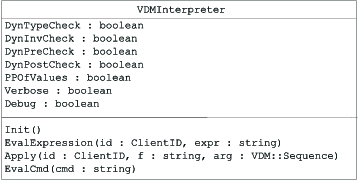
\includegraphics{VDMInterpreter.png}}
\caption{The {\tt VDMInterpreter} interface.}\label{fig:VDMInterpreter}
\end{center}
\end{figure}

%\begin{figure}[tbh]
%\begin{center}
%\begin{tabular}{|l|}
%\hline
%{\tt ToolboxAPI::VDMInterpreter } \\
%\hline
%{\tt DynTypeCheck: boolean } \\
%{\tt DynInvCheck: boolean } \\
%{\tt DynPreCheck: boolean } \\
%{\tt DynPostCheck: boolean } \\
%{\tt PPOfValues: boolean } \\
%{\tt Verbose: boolean } \\
%{\tt Debug: boolean } \\
%\hline
%{\tt Initialize () } \\
%{\tt EvalExpression (in VDM::ClientID id, in string expr) } \\
%{\tt Apply (in VDM::ClientID id, in string f, in VDM::VDMSequence arg) } \\
%{\tt EvalCmd (in string cmd) } \\
%{\tt SetBreakPointByPos (in string file, in long line, in long col) } \\
%{\tt SetBreakPointByName (in string mod, in string func) } \\
%{\tt DeleteBreakPoint (in long num) } \\
%{\tt StartDebugging (in VDM::ClientID id, in string expr) } \\
%{\tt VDM::VDMTuple DebugStep (in VDM::ClientID id) } \\
%{\tt VDM::VDMTuple DebugStepIn (in VDM::ClientID id) } \\
%{\tt VDM::VDMTuple DebugSingleStep (in VDM::ClientID id) } \\
%{\tt VDM::VDMTuple DebugContinue (in VDM::ClientID id) } \\
%\hline
%\end{tabular}
%\caption{The {\tt VDMInterpreter} interface.}\label{fig:VDMInterpreter}
%\end{center}
%\end{figure}

The {\tt \VDMInterpreter} interface is shown in
Figure~\ref{fig:VDMInterpreter}. This interface allows you to use the
interpreter to evaluate and debug VDM expressions and invoke functions and
operations in the specification. Calling {\tt EvalExpression(client\_id, expr)}
will evaluate the expression in the string argument {\em expr} and
return the result to the client. The result will be represented as the
VDM value {\tt \Generic} described in
Section~\ref{idldescriptionvalues}. For instance,

\newpage
\begin{quote}
\begin{verbatim}    
EvalExpression(client_id, "[e | e in set {1,...,20} 
             & exists1 x in set {2,...,e} & e mod x = 0 ] ")
\end{verbatim}
\end{quote}

would return a {\tt \Generic} holding the sequence of all primes
between one and twenty. 
Alternatively one could specify (in VDM) a more efficient function,
{\tt Primes}, for extracting all primes from a sequence and invoke it
through the {\tt Apply} method of the interface: 

\begin{quote}
\begin{verbatim}    
Apply(client_id, "Primes", s)
\end{verbatim}
\end{quote}

with {\tt s} being the argument for the function. {\tt Apply} will
also return the result of applying the function to the given arguments
as a VDM value contained in an {\tt \Generic}. 
(In fact this example is a slight simplification of how to pass 
arguments for a function when using {\tt Apply}. 
We  will describe the correct way to use {\tt Apply} in Section~\ref{cpp:interp} 
for C++ clients, and Section~\ref{java:interp} for Java clients.

In this example it is convenient to use the interpreter to construct
the sequence of integers: 

\begin{quote}
\begin{verbatim}    
s = EvalExpression(client_id, "[e|e in set {1,...,20}]")
\end{verbatim}
\end{quote}

and use the returned value {\tt s} as argument to {\tt
  Apply}. Alternatively the client could have manually constructed the
sequence. 

Apart from the functions already mentioned, the interpreter interface
holds a number of attributes (boolean values) that can be modified
from the client. The settings of these attributes control the way the
interpreter behaves.  The first five attributes ({\tt DynTypeCheck},
{\tt DynInvTheck}, {\tt DynPreCheck}, {\tt DynPostCheck}, {\tt
  PPOfValues}) corresponds to the options for the interpreter that it
is possible to set from the user interface of the VDM Toolbox. They
control aspects such as dynamic type checking of invariants, pre- and
post conditions etc.  The two remaining attributes, {\tt Verbose} and
{\tt Debug}, control how the API uses the interpreter. {\tt Verbose}
controls whether or not the result of using the interpreter should be
echoed in the user interface of the VDM Toolbox. If {\tt Verbose} is
false the client will use the interpreter ``silently" without echoing 
results to the user interface.  The attribute {\tt Debug} controls
whether breakpoints in the specification are respected during
evaluation or not. If {\tt Debug} is set to true the evaluation will
be suspended at each breakpoint and the user is able to debug the
specification. In this case the call to {\tt Apply} and {\tt
  EvalExpression} will not return before the user has finished the
debugging. 

It is possible to set breakpoints using the methods {\tt SetBreakPointByPos}
and {\tt SetBreakPointByName}. While the first method takes a file and
a position (line, column) as parameters, the latter expects the name of the
module and a function name. Both methods return the number of the breakpoint
that has been set. This number can be used to delete the breakpoint again
({\tt DeleteBreakPoint}).

Debugging is then started by calling {\tt StartDebugging}. The method takes
the {\tt ClientID} and an expression (a string) as parameter. {\tt StartDebugging}
returns, when the evaluation is finished or a breakpoint has been encountered.
It returns a {\tt VDMTuple}, containing the evaluation state (either
{\tt <BREAKPOINT>}, {\tt <INTERRUPT>}, {\tt <SUCCESS>} or {\tt <ERROR>}) and,
in case of {\tt <SUCCESS>}, the result of the evaluation as a MetaIV value.
The methods {\tt DebugStep}, {\tt DebugStepIn}, {\tt DebugSingleStep} and 
{\tt DebugContinue} can be used to step through the specification.

Assume we have a module \texttt{A} that contains two functions:

\begin{verbatim}
module A
  ...
  functions
     foo: nat -> nat
     foo (a) == a + 1;

     bar: nat -> nat
     bar (b) = foo (b)
  ...
\end{verbatim}

We could use {\tt SetBreakPointByName ("A", "foo")} to set a 
breakpoint for the function {\tt foo}. The call of
{\tt StartDebugging (id, "A`bar(1))} would then return after 
the call of {\tt foo (b)} in {\tt bar} has been encountered.
The result would be {\tt mk\_( <BREAKPOINT>,<<UNDEFINED>> )}.
A call to {\tt DebugContinue} continues the evaluation and
would return {\tt mk\_( <SUCCESS>, 2 )}.

\subsubsection{VDMErrors}
\label{VDMErrors}

\begin{figure}[tbh]
\begin{center}
\mbox{}
\resizebox{8cm}{!}{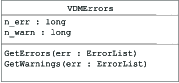
\includegraphics{VDMErrors.png}}
\caption{The {\tt VDMErrors} interface.}\label{fig:VDMErrors}
\end{center}
\end{figure}

%\begin{figure}[tbh]
%\begin{center}
%\begin{tabular}{|l|}
%\hline
%{\tt ToolboxAPI::VDMErrors } \\
%\hline
%{\tt NumErr: short } \\
%{\tt NumWarn: short } \\
%\hline
%{\tt GetErrors(out ErrorList err) } \\
%{\tt GetWarnings(out ErrorList err) } \\
%\hline
%\end{tabular}
%\caption{The {\tt VDMErrors} interface.}\label{fig:VDMErrors}
%\end{center}
%\end{figure}

The {\tt \VDMErrors} interface is shown in Figure~\ref{fig:VDMErrors}.
The state of this interface is updated if errors are encountered
during parsing, type checking, code generation or pretty printing. Use
this interface to query the number of errors and/or warnings through
the attributes {\tt n\_err} and {\tt n\_warn}. The two methods of the
interface return a sequence of error or warning descriptors used to
gain detailed information.

\subsection{IDL Description of VDM Values}
\label{idldescriptionvalues}

Having described the interface of the VDM Toolbox, we will now proceed
with a description of how VDM values are passed through the API,
i.e. how VDM values can be passed from the VDM Toolbox to the client
and vice versa. 

The given code examples are written in C++. We refer to
section~\ref{writingajavaclient} for the Java syntax.

As already mentioned, the {\tt EvalExpression} method of the {\tt
  \VDMInterpreter} interface returns the result of the evaluation as a
VDM value, and the {\tt Apply} method takes as argument a VDM sequence
of VDM values as the list of arguments for a function or operation.
How to use and manipulate such VDM values is documented in Section~\ref{ref:vdmapi}
and also described in the IDL file {\tt metaiv\_idl.idl}. The structure of
the IDL interface is kept as tight as possible to the structure of the
VDM C++ Library (as described in \cite{LibMan-CSK}).  Each class of the
VDM C++ Library corresponds to an interface (with the same name) in
the IDL description. Figure~\ref{fig:VDMvalues} illustrates the fact
that all concrete VDM values inherit from the same super class, {\tt
  \Generic}.  Notice that the figure only shows a subset of the
available VDM values.

\begin{figure}[tbh]
\begin{center}
\mbox{}
\resizebox{14cm}{!}{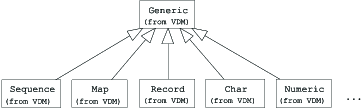
\includegraphics{VDMvalues.png}}
\caption{Inheritance structure of VDM values.}\label{fig:VDMvalues}
\end{center}
\end{figure}

The following is an example of how to read the contents of a VDM value
returned from the interpreter: 

\begin{verbatim}
01  VDM::VDMGeneric_var g;
02  g = interp->EvalExpression(client_id, 
                            "{ e |-> 2**e | e in set {1,...,16}}");
03  if(!g->IsMap()){
04    // signal an error...
05    ...
06  }
07  else{
08    VDM::VDMMap_var m;
09    m = VDM::VDMMap::_narrow(g);
10    VDM::VDMGeneric_var iter;
11    for(int i = m->First(iter); i; i = m->Next(iter)){
12      VDM::VDMGeneric_var rng = m->Apply(client_id, iter);
13      cout << iter->ToAscii() << "-->" << rng->ToAscii() << "\n"; 
14      iter->Destroy();
15      rng->Destroy();
16    }
17  }
18  g->Destroy();
\end{verbatim}

The interpreter returns the result of an evaluation in a {\tt
  \VDMGeneric}. For this reason the variable {\tt g} is declared as a {\tt
  VDM::Generic\_var}\footnote{See Section~\ref{writingacppclient} for
  a description of the special {\tt \_var} types used in the client
  and how to use CORBA object references.}, and used to hold the
  result from 
{\tt EvalExpression}. The expression evaluated by the interpreter is a map
comprehension; hence the value contained in {\tt g} should be of type
  {\tt \Map}. 
The method  {\tt IsMap} of the {\tt \Generic} interface can be used to
check that this is indeed the case, as seen in line 3. If {\tt g} is
not of type {\tt \Map} an 
error is signalled. Otherwise it is safe to convert the {\Generic} to a
 {\Map} type. The way to cast (or narrow) an object reference is to use
the {\tt \_narrow} method supplied by the ORB implementation. Line 9
shows how to narrow from {\tt \VDMGeneric} to {\tt \VDMMap}. With an object
reference, {\tt m}, of type  {\tt \VDMMap} all the methods of the {\Map}
interface 
are now available. Using {\tt First} and {\tt Next} it is possible to iterate
through the domain of the map (line 11), and with {\tt Apply} (line 12) the
value associated with a key in the map can be retrieved. 
Keep in mind, that only \emph{one} Client should access these methods
at a time. If you use them concurrently, the clients may not get all
values contained by the {\tt VDMMap}.

To facilitate
the printing of VDM values, the {\Generic} interface (and hence all other
VDM values) provides the {\tt ascii} method returning the ASCII
representation of the VDM value. In line 13 this method is used to
print out each element of the map {\tt m}. 

To summarize: This simple
example uses the interpreter to construct a map that is subsequently
printed using the various methods of {\tt \VDMMap} to iterate through the
map. The output from the example above is: 

\begin{quote}
\begin{verbatim}    
1-->2 
2-->4 
3-->8 
... (lines removed for brevity) ...  
16-->65536
\end{verbatim}
\end{quote}

\subsubsection{VDM Values as Distributed Objects}

Whenever VDM values are passed from the server to the client they are
passed as ``handles" or object references to distributed objects
contained in the server. That is, the real VDM values used by a client
are actually managed by the VDM Toolbox and are contained in the address
space of the server. For this reason {\em all} VDM values held by a
client must be 
explicitly freed in the server when the client will not use the value
any longer. The client does this by calling the {\tt Destroy} method
of the VDM value. In lines 14 and 15, of the example above, the object
{\tt iter}, used to represent each element in the domain of {\tt m},
and {\tt rng}, used to hold the corresponding element of the range of
{\tt m}, are destroyed. Finally, in line 18 the VDM value created by
the interpreter, {\tt g}, is destroyed. If values are not destroyed in this
way when the client does not need them any more, they will never be
released in the VDM Toolbox. As a consequence the VDM Toolbox process
will use an increasing amount of memory.  

An alternative to explicitly destroy objects by calling the {\tt Destroy}
method on the object is to use the two methods {\tt PushTag} and {\tt
  DestroyTag} 
of the {\tt \VDMApplication} interface. Calling {\tt PushTag} will generate a
unique tag and push it onto an internal tag stack. The tag stored on
top of the tag stack is used to tag all objects subsequently created
by the VDM Toolbox. Each call to {\tt DestroyTag} will pop the topmost tag
of the tag stack and call destroy on each object tagged with this
value. As a consequence all objects created since the last call to
{\tt PushTag} will be destroyed.  Using the combination of {\tt PushTag} and
{\tt DestroyTag} the previous example now reads as follows:

\begin{verbatim}
01  app->PushTag(client_id);
02  VDM::VDMGeneric_var g;
03  g = interp->EvalExpression(client_id, 
                            "{ e |-> 2**e | e in set {1,...,16}}");
04  if(!g->IsMap()){
05    // signal an error...
06    ...
07  }
08  else{
09    VDM::VDMMap_var m;
10    m = VDM::VDMMap::_narrow(g);
12    VDM::VDMGeneric_var iter;
12    for(int i = m->First(iter); i; i = m->Next(iter)){
13      VDM::VDMGeneric_var rng = m->Apply(client_id, iter);
14      cout << iter->ToAscii() << "-->" << rng->ToAscii() << "\n"; 
15    }
16  }
17  app->DestroyTag(client_id); 
                 // All objects created since last PushTag()
                 // will now be destroyed.
\end{verbatim}

Notice that calls to {\tt PushTag} and {\tt DestroyTag} can be nested
to any depth as long as the total number of calls to {\tt DestroyTag}
does not exceed the total number of calls to {\tt PushTag}. 

\subsubsection{Using Values Returned from the Interpreter}

In the example above we used the {\tt ToAscii} method to print the range
and domain of the map generated by the interpreter. The value, as
opposed to the ASCII representation, is available through the {\tt
  GetValue} method. For instance, the following code squares each
element of a sequence and prints out the result: 

\begin{verbatim}
01  app->PushTag(client_id);
02  g = interp->EvalExpression(client_id, 
                               "[ e | e in set {1,...,10}]");
03  if(!g->IsSequence()){
04    exit(-1);
05  }
06  else{
07    VDM::VDMSequence_var s = VDM::VDMSequence::_narrow(g);
08    for(int i = 1; i <= s->Length(); i++){
09      VDM::VDMGeneric_var e = s->Index(i);
10      if(e->IsNumeric()){
11        VDM::VDMNumeric_var ii = VDM::VDMNumeric::_narrow(e);
12        cout << ii->GetValue() * ii->GetValue() << " ";
13      }
14    }
15  }
16  app->DestroyTag(client_id);
\end{verbatim}

Notice that the  {\tt PushTag} and {\tt DestroyTag} methods are also
used in this example to make sure that values used by the client are
released in the VDM Toolbox when the client no longer needs them.  

In what follows we will assume that all code examples are ``wrapped"
with calls to {\tt PushTag} and {\tt DestroyTag}, so that we will not
have to call {\tt Destroy} explicitly.

\subsubsection{Constructing VDM Values in the Client}

The VDM values we have used so far were all created by the interpreter
and returned to the client. However, the client can construct VDM
values directly by using the {\tt \VDMFactory} interface. The following
example acquires a handle to the {\tt \VDMFactory} interface and constructs a
set of numeric values:

\begin{verbatim}
VDM::VDMFactory_var fact = app->GetVDMFactory();
VDM::VDMSet_var s = fact->MkSet(client_id);
VDM::VDMNumeric_var elem;
for(int j=0; j<20; j++){
  elem = fact->MkNumeric(client_id, j);
  s->Insert(elem);
}
\end{verbatim}

Notice that the factory interface is used to construct the overall set
as well as each numeric value to be inserted in the set. Also notice
that each numeric value constructed by the factory is destroyed after it has
been inserted in the set, because elements are implicitly copied when
inserted into composite types such as {\tt \VDMSequence}, {\tt
  \VDMSet}, {\tt \VDMMap}, {\tt \VDMRecord} and {\tt \VDMTuple}. 

\subsubsection{Converting Distributed VDM Values to ``real" VDM C++ Values}

It is important to keep in mind that when the client receives a VDM
value from the interpreter, it is simply holding a handle to a VDM 
value contained in the VDM Toolbox. Every time the client invokes a
method on the VDM value this method call is mediated to the
distributed VDM value in the VDM Toolbox. For this reason, when the
client iterates through, for instance, a large sequence returned from
the interpreter, the VDM Toolbox gets called for each element in the
sequence. Of course this approach is not particularly efficient. To
allow more efficient access to VDM values held by the client, you can
use 
%the function {\tt GetCPPValue} of the {\tt \Generic} interface, or
%(as in the example below), 
the function {\tt GetCPPValue} declared in
the file \texttt{corba\_client.h}. This
function converts the distributed VDM value to an IDL sequence of
bytes, which can in turn be converted to a true VDM C++ value,
provided that you include {\tt metaiv.h} and link with the VDM
library \cite{LibMan-CSK}. For ease of use the conversion from a distributed VDM value
to a VDM C++ value is available in {\tt corba\_client.h}. Simply call
{\tt GetCPPValue} and give it as argument the object reference you
wish to convert:
\begin{verbatim}
#include "metaiv.h"

g = interp->EvalExpression(client_id, "[ e | e in set {1,...,10}]");
Generic cpp_g;  // The C++ Generic
cpp_g = GetCPPValue(g);
// Now the C++ value cpp_g is local to the client process and can
// be accessed efficiently. 
\end{verbatim}

The conversion from a VDM C++ value to an object reference can be
achieved through the function {\tt FromCPPValue}, also declared, as
well as documented, in {\tt corba\_client.h}.  

For Java clients, the conversion described above has to be done
manually, and the VDM Java Library must be included in the classpath
when compiling and executing the client \cite{CGJavaManPP-CSK}.
See the function \texttt{EchoPrimes2} in the Java program in
Appendix~\ref{A4} for an example.

\subsection{Handling of Exceptions}
\label{handlingofexceptions}

The IDL interface {\tt metaiv\_idl.idl}  declares two CORBA exceptions
{\tt APIError} and {\tt VDMError}. These two kinds 
of exceptions are used to signal to the client process if something
goes wrong in the server process. {\tt APIError} is used to signal errors
that may appear while using the API of the VDM Toolbox ({\tt
  corba\_api.idl}) while {\tt VDMError} is devoted to the signalling of
errors in the use of VDM values. The contents of an {\tt APIError} is a
simple message string describing what went wrong, while a {\tt VDMError}
holds an integer indicating the error. The meaning of these integers
is shown in Section~\ref{ref:exceptions}.

The examples in Appendix~\ref{A3} and ~\ref{A4} show how
the client can handle such exceptions using standard exception
handling in C++ and Java respectively.

\newpage
\section{Writing a C++ Client}
\label{writingacppclient}

We will here describe  how to write a client using C++ on Windows
and Linux.  

\subsection{Choosing a CORBA Implementation}

The CORBA implementation we will use in this example is a CORBA 2
compliant ORB {\em omniORB3}. The implementation is developed by {\em The
AT\&T Laboratories Cambridge}, and freely available under
the terms and conditions of the GNU General Public License. Several
platforms and C++ compilers are supported by omniORB3 that implements
a full mapping from IDL to C++.  The ORB can be downloaded from:

\begin{quote}
\begin{verbatim}    
http://www.uk.research.att.com/omniORB/omniORB.html
\end{verbatim}
\end{quote}

and available as pure C++ source code or pre-compiled for a handful of
different platforms 
including Windows 2000/XP/Vista and Linux 2.4 or 2.6. If the distribution is not
available for a particular platform it is possible to download the
source code and build the executables and libraries.  

To implement a
client you must download the onmiORB3 distribution for either Win32 or
Linux and install it (extract the archive). Once omniORB is installed
you should add to the system path environment variable the absolute
path to the binaries directory of omniORB. This directory contains
various CORBA tools (the IDL compiler for instance). For the Windows
2000/XP/Vista distribution it also contains some libraries used by the client
implementation at run-time. If you download the pre-compiled
distribution this is all you need to do. Otherwise you must consult
the installation instructions of omniORB to successfully compile the
distribution.  

Alternatives to omniORB would be e.g. {\em Orbacus} by 
{\em Object Oriented Concepts} and the {\em idlj} from Sun's Java IDL. Any
ORB that implements the OMG CORBA 2.x specification and IIOP should be
compatible with the VDM Toolbox API, but this has not been tested.

Orbacus implements a complete mapping from IDL to
C++ as well as Java, so this ORB may be the choice it you wish to
write your client in Java. Orbacus is available at:

\begin{quote}
\begin{verbatim}    
http://www.ooc.com/ob/ 
\end{verbatim}
\end{quote}


Java IDL comes with an IDL to Java compiler and is available
at

\begin{quote}
\begin{verbatim}    
http://java.sun.com 
\end{verbatim}
\end{quote}

However, the client example distributed with
the VDM Toolbox (listed in Appendix~\ref{A3}) is omniORB3 specific, so
if OmniBroker is used, slight modifications of the client example are
required.

\subsection{Implementing a Client}

In this Section we go through an example illustrating how to use the
VDM Toolbox from a client written in C++. In the following
presentation we will show excerpts from a complete example, which can
be seen in its full length in Appendix~\ref{A3}.  

\subsubsection{Initializing the CORBA Services}

Before the VDM Toolbox can be accessed from the client the underlying
CORBA implementation must be initialized. Different CORBA
implementations are not necessarily initialized in the same way, so
please notice that the CORBA initialization described here is omniORB
specific. For ease of use the initialization procedure and the
acquisition of the main application object are implemented in {\tt
  corba\_client.cc} and available by including {\tt corba\_client.h}
in the client implementation. If you wish to implement the client on a
different CORBA implementation it should not be too difficult to port
the contents of {\tt corba\_client.cc}. You will find
\texttt{corba\_client.cc} and \texttt{corba\_client.h} in the
\texttt{api/corba} subdirectory of the VDM Toolbox distribution.

To initialize the CORBA services all you need to do is:

\begin{verbatim}
#include "corba_client.h"

main(int argc, char *argv[])
{
  init_corba(argc, argv);
  ...
}
\end{verbatim}

\subsubsection{Acquiring the Application Object}

The easiest possibility to get hold of a CORBA-reference to
the VDMApplication CORBA object is to use the {\tt get\_app} method
that you can find in the above mentioned \texttt{corba\_client.h} 
file. Since the implementation is omniORB-specific, this may
not work with the ORB of your choice. Therefore, the COS NamingService
and stringified references are supported, too.

The COS NamingService is a standardized CORBA Object Service that
is used for managing object instances and their names. It maps
names, that are saved in a directory hierarchy to CORBA Objects.
Unlike the stringified object references it allows the client
to access objects even if it doesn't share the file system with
the VDM Toolbox. Therefore by using it, you gain flexibility. Its
use is recommended by the Object Management Group (\texttt{http://www.omg.org)}.
You can find more information on the COS NamingService and 
CORBA Object Services in general on the OMG CORBA homepage 
(\texttt{http://www.corba.org}).

When you start either the VDM-SL or the VDM++-Toolbox, it will
check if a COS NameService is running. The ORB will search for
a configuration file. You can specify the location of this
file using the {\tt OMNIORB\_CONFIG} environment variable (refer
to the omniORB-documentation to see how to use the registry for
this if you use Windows). A typical {\tt omniORB.cfg} file
will contain following entries:

\begin{verbatim}
ORBInitialHost gandalf
ORBInitialPort 2809
\end{verbatim}

This means, that the NamingService is running on a host
called {\tt gandalf} at port 2809.

omniORB provides such a
NameService (there should be an executable called \texttt{omniNames}
that is part of the omniORB-distribution), but you can use
virtually any other CORBA-compliant NameService as long as you
make it known to the omniORB using the \texttt{omniORB.cfg} file.
Please refer to the omniORB documentation for further details.
The VDM-SL Toolbox binds its {\tt VDMApplication} object to the name
{\tt SL\_TOOLBOX}, of kind {\tt VDMApplication}, while Application object of the
VDM++ Toolbox uses the name {\tt PP\_TOOLBOX}, of kind {\tt VDMApplication}. This
makes it possible for the client to distinguish the objects, so
that it is no problem to run an instance of each Toolbox at the
same time. 

Take care that you do not run two instances of the
same Toolbox, because then only the {\tt VDMApplication} object
of the Toolbox that has been started first will be accessible
for the client. It is no problem to run more than one client
using the same {\tt VDMApplication} object, but keep in mind
that they will influence each other.

Another approach used to acquire the main handle to the VDM Toolbox - the
{\tt VDMApplication} CORBA object - is to let the client read a stringified
object reference (created by the most recently started VDM Toolbox)
and convert this to a CORBA object reference. All ORB implementations
must implement the two functions {\tt object\_to\_string} and {\tt
  string\_to\_object}, used to encode and decode object references.
The VDM Toolbox uses {\tt object\_to\_string} to encode the
application object as a string and writes this string to a file.
Subsequently the client must read this file and use {\tt
  string\_to\_object} to convert the string to an object reference.
 The file generated by the VDM Toolbox is named {\tt
  vdmref.ior} for the VDM-SL Toolbox and {\tt vppref.ior} for
the VDM++ Toolbox. It is written in the location specified by the
{\tt VDM\_OBJECT\_LOCATION} environment variable.
If the environment variable is not set, the file is 
located in the root of your home directory (as pointed to by {\tt
  \$HOME}) if the VDM Toolbox is running on Unix, and in your profile
directory (as pointed to by {\tt \%USERPROFILE\%}) if running on Windows 2000/XP/Vista.

The easiest way to acquire the application object from the client is
to use {\tt get\_app} declared in {\tt corba\_client.h}.

\begin{verbatim}
main(int argc, char *argv[])
{
 ...
 /* set toolType to either SL_TOOLBOX or PP_TOOLBOX */
 ToolType toolType = ...;
 VDMApplication_var app;
 get_app(app, NULL, toolType);
 ...
\end{verbatim}

This function will check first, if a COS NameService is running
and if there is an object named {\tt SL\_TOOLBOX} of kind {\tt VDMApplication}
or {\tt PP\_TOOLBOX}, kind {\tt VDMApplication} (depending on the {\tt toolType} flag).
If it cannot find the object via the NameService, it will
will automatically search for the file that
contains the IOR reference for the {\tt VDMApplication} object. 
After the call to {\tt get\_app} the variable
{\tt app} is the main handle to the VDM Toolbox.

The client has to register itself in the server before performing any
calls towards the server. Analogously, it has to unregister itself
when it terminates. This is done by calling the  {\tt Register} and
{\tt Unregister} methods of the {\tt \VDMApplication} class. 

\begin{verbatim}
client_id = app->Register();
...
app->Unregister(client_id);
\end{verbatim}

We are now in the position to access services of the running VDM Toolbox.

\subsubsection{Object References in C++}
\label{objectreferences}

In C++ a handle to an object interface of the IDL description is
contained in an {\em object reference}. Object references are named by
adding {\tt \_var} to the name of the interface. This kind of object
reference is termed an {\em object reference variable}\footnote{Object
references are also available in a more simple form, the {\tt \_ptr}
object references. We refer to \cite{omniORB3} and \cite{OMG&96} for
more information on the difference between the two types of object
references. For most purposes it is sufficient to use only the {\tt
\_var} object references.}. For instance, {\tt 
VDMApplication\_var} is a handle (if properly initialized) to the 
{\tt \VDMApplication} interface of the server. Operations of an interface are
called using the ``arrow" ({\tt ->}) on a {\tt \_var} object reference, e.g.
{\tt app->GetProject()} to call the method {\tt GetProject} of the
{\tt \VDMApplication} interface {\tt app}.

\subsubsection{Configuring the Current Project}

The following lines of code acquire a handle to the {\tt \VDMProject}
interface of the VDM Toolbox and use the {\tt New} and {\tt AddFile} methods of
this interface. As a result the project of the VDM Toolbox is
configured to contain a single file, {\tt sort.vdm}. Files added to the
project in this way must be located in the same directory as where the
VDM Toolbox was started. Otherwise the file name must be given with
its absolute path. If the client tries to add a non-existing file the
server will throw an exception of type {\tt APIError} indicating the error.
These exceptions are described in Section~\ref{handlingofexceptions}.

\begin{verbatim}
VDMProject_var prj = app->GetProject();
prj->New();  // New project
prj->AddFile("sort.vdm");
\end{verbatim}

\subsubsection{Using the Parser}
To use the parser from a client you must get a handle to the {\tt \VDMParser}
interface, and to parse a file you call the {\tt Parse} method of this
interface with the file name as its single argument. For instance
\begin{verbatim}
VDMParser_var parser = app->GetParser();
parser->Parse("sort.vdm");
\end{verbatim}
will parse the file {\tt sort.vdm}.

Alternatively you could use the {\tt \VDMProject} interface to get the
list of files configured for the current project and then parse each
file of this list:

\begin{verbatim}
FileList_var fl;
prj->GetFiles(fl);

for(int i=0; i<fl->length(); i++){
  cout << (char *)fl[i] << "...Parsing...";
  if(parser->Parse(fl[i]))
    cout << "done.\n";
  else
    cout << "error.\n";
}
\end{verbatim}

This example illustrates several important aspects of the API.
Initially we declare {\tt fl} to be a list of files and use {\tt GetFiles}
to retrieve the list of files in the current project. 
The type {\tt \FileList} is defined
as an unbounded sequence of strings, as shown on page
\pageref{ref:corbatypes}. Consequently the list of files,
{\tt fl}, has all methods of the IDL sequence as stated by the CORBA
specification \cite{OMG&96}. The length of a IDL sequence can be accessed
through the method {\tt length}, and the individual elements can be indexed
as ordinary arrays in C++.  

To summarize: The above lines of code
retrieve the list of files in the current project, iterate through the
list, and for each item calls the {\tt Parse} method to parse each file.
Notice that {\tt Parse} returns a boolean value indicating the success of
parsing the file.  Parsing all files of the project by iterating the
list of files is actually more complicated than need to be. Instead
you could use the {\tt ParseList} method:

\begin{verbatim}
FileList_var fl;
prj->GetFiles(fl);
parser->ParseList(fl);
\end{verbatim}

\subsubsection{Using the Type Checker}
\label{usingthetypechecker}

The interface of the type checker is similar to the interface
of the parser. The interface has a number of attributes that can be
accessed and modified by the client. Attributes can be read and
modified for example: 

\begin{verbatim}
// Get the value of DefTypeCheck:
int dtc = tpck->DefTypeCheck();

// Set the value of ExtendedTypeCheck to true
tpck->ExtendedTypeCheck(true);
\end{verbatim}

provided of course that \texttt{tpck} is a valid handle to the type
checker interface.  

\subsubsection{Using the Interpreter}\label{cpp:interp}
\label{usingtheinterpreter}

The following example illustrates how {\tt EvalExpression} of the
interpreter interface can be used to have the interpreter evaluate any
VDM expression.

\begin{verbatim}
VDMInterpreter_var interp = app->GetInterpreter();
VDM::Generic_var g;

g = interp->EvalExpression(client_id, "[e|e in set {1,...,20} & \
  exists1 x in set {2,...,e} & e mod x = 0 ]");

if(g->IsSequence())
  cout << "All primes below 20:\n" << g->ascii() << "\n";
\end{verbatim}

The string passed to {\tt EvalExpression} is evaluated and the result
  of the evaluation is returned as a VDM value in a {\tt VDM::Generic},
  which can later be used in a call to {\tt Apply}, or read/modified by the
  methods provided by the interface of the VDM values as described in
  Section~\ref{idldescriptionvalues}. The backslash at the end of the
  line in which the call to \texttt{EvalExpression} is placed is part
  of the C++ 
  syntax. It is used to indicate, that the string that contains the 
  VDM-SL expression does not contain a linebreak (\verb+\n+). 

The following example illustrates how to use a function of a VDM
specification that has been read into the VDM Toolbox: 

\begin{verbatim}
interp->Init();
g = interp->EvalExpression(client_id, "MergeSort([6,4,9,7,3,42])");
\end{verbatim}

Notice that before you can call any function of the specification you
must make sure that the interpreter is initialized.  

An alternative to {\tt EvalExpression} is to use the method {\tt
  Apply}, which takes as argument the name of the function or
operation to apply and a sequence of arguments for the function or
method. The following example creates a VDM sequence of integers to be
sorted with {\tt MergeSort}:

\begin{verbatim}
VDMFactory_var fact = app->GetVDMFactory();
    
VDM::Sequence_var list = fact->MkSequence(client_id);
VDM::Int_var elem;
for(int j=0; j<20; j++){
  elem = fact->MkInt(client_id, j);
  list->ImpPrepend(elem);
}
\end{verbatim}

The resulting sequence, {\tt list}, now contains the integers from 19
down to 0. Notice how VDM values are constructed in the client by
using the {\tt \VDMFactory} interface.  

To call {\tt MergeSort} through {\tt Apply} we
have to construct the list of arguments. The arguments for the
function to be called through {\tt Apply} are contained in a {\tt
  \VDMSequence}. 
The function we want to call only takes one argument, the sequence of
integers we have just constructed:

\begin{verbatim}
VDM::Sequence_var arg_l = fact->MkSequence(client_id);
arg_l->ImpAppend(list);
\end{verbatim}

Now \texttt{MergeSort} can be applied as follows:

\begin{verbatim}
g = interp->Apply(client_id, "MergeSort", arg_l);
\end{verbatim}

if, of course, the interpreter has been initialized. Notice that the
argument list {\tt arg\_l} is also constructed using the factory
interface.  

\subsubsection{Additional Aspects of the Example}

So far we have covered most of the example from Appendix~\ref{A3}. Also
covered in this example is how detailed error information can be
queried through the API and how to get additional information on the
status of individual modules. We will not go into further details with
the example here, but refer to the interfaces {\tt \VDMErrors} and
{\tt \VDMModuleRepos} of the IDL description as well as the example source
code and comments of Appendix~\ref{A3} for more information.

\subsection{Compiling the Client}

To successfully compile the file {\tt client\_example.cc} each of the
following requirements must be fulfilled: 

\begin{itemize}
\item The omniORB must have been successfully installed
  If the binary 
  distribution is not available for your particular platform it must
  be compiled as well. Moreover, the {\tt PATH} environment variable
  must point to the binaries directory of omniORB.

\item 
The following files, found in \texttt{\$TOOLBOX/api/corba},
must be present (where \texttt{\$TOOLBOX} represents the directory in
which the Toolbox was installed).
\begin{itemize}
\item {\tt client\_example.cc}
\item {\tt corba\_client.h}, {\tt corba\_client.cc}
\item {\tt corba\_api.idl}, {\tt metaiv\_idl.idl}
\item {\tt Makefile}, {\tt Makefile.nm}
\end{itemize}

\item
Your VDM Toolbox must contain the VDM C++ library, i.e. the include
file {\tt metaiv.h} and the library {\tt libvdm.a} (Unix) or {\tt
vdm.lib} (Windows 2000/XP/Vista). 
\end{itemize}

To compile the example you can simply use the makefile. On Linux 
you run {\tt make} with {\tt Makefile},
while on Windows 2000/XP/Vista you use {\tt nmake} with {\tt Makefile.nm}. You
must modify the macros {\tt OMNIDIR} and {\tt TBDIR} of the make file
to point to the installation directory of omniORB and the VDM Toolbox
respectively. 

Note that if you wish to use Microsoft's Foundation Classes under
win32, the MFC library should be statically linked.

\subsubsection{Supported Compilers}

The client example in Appendix~\ref{A3} has been compiled and tested
on Microsoft Windows 2000/XP/Vista and Microsoft Visual C++ 2005 SP1, 
and on Linux with GNU gcc 3, 4.

\subsection{Running the Client}
Before you run the client example you must ensure that a VDM Toolbox
to be used as server is currently running. Use the {\tt
  VDM\_OBJECT\_LOCATION} environment variable in order to tell the
client where to look for the {\tt [vdm|vpp]ref.ior} file.

\newpage
\section{Writing a Java Client}
\label{writingajavaclient}

\subsection{Choosing a CORBA Implementation}

The Java 1.3 API contains a package called {\tt org.omg.CORBA}, that
provides the mapping of the OMG CORBA APIs to the Java programming
language. The package includes the class {\tt ORB}, which is
implemented so that a programmer can use it as a fully-functional
Object Request Broker. 

The example in the following will use this CORBA implementation. 

In addition to a CORBA implementation, the user needs to have access
to the described IDL modules: {\tt corba\_api.idl} and {\tt
  metaiv\_idl.idl}. These have been translated to Java packages and
classes and can be used by including the {\tt ToolboxAPI.jar} file in
the classpath. This file is part of the Toolbox distribution, in the
\verb+api/corba+ sub-directory. 

It contains three packages:

\begin{itemize}
\item  {\tt jp.co.csk.vdm.toolbox.api.corba.VDM}
  
  This package contains the VDM module defined in {\tt
    metaiv\_idl.idl}. It contains
  consequently a Java interface for every VDM value.

\item {\tt jp.co.csk.vdm.toolbox.api.corba.ToolboxAPI} 
  
  This package contains the interfaces from {\tt corba\_api.idl}.

\item {\tt jp.co.csk.vdm.toolbox.api} 
  
  This package contains only one class, called {\tt ToolboxClient}. It
  implements methods used to connect client applications to the
  VDM Toolbox through the VDM Toolbox CORBA API. 
\end{itemize}

All three packages are documented by HTML documentation generated by
the {\em javadoc} program. Both the {\tt ToolboxAPI.jar} file and the
HTML documentation are distributed with the VDM Toolbox. 

If you don't use the CORBA implementation following with Java 1.3, you
have to translate the IDL files to Java yourself. The files in
\texttt{ToolboxAPI.jar} have been created using the {\tt idltojava}
compiler (downloadable from the Java Developer Connection): 
\verb+http://developer.java.sun.com+. If you are using the Sun JDK 1.3
an executable {\tt idlj} will be part of the distribution. It is the
SUN IDL to Java compiler, that generates the Java stubs and skeletons
for you.


\subsection{Implementing a Client}

In this Section we go through an example illustrating how to use the
VDM Toolbox from a client written in Java. In the following
presentation we will show excerpts from a complete example, which can
be seen in full length in Appendix~\ref{A4}. 

\subsubsection{Importing CORBA Services}

Your client program should start by importing the {\tt org.omg.CORBA}
package together with the three packages described above:

\begin{verbatim}
import org.omg.CORBA.*;

import jp.co.csk.vdm.toolbox.api.ToolboxClient;
import jp.co.csk.vdm.toolbox.api.corba.ToolboxAPI.*;
import jp.co.csk.vdm.toolbox.api.corba.VDM.*;
\end{verbatim}

%Though capitalized, {\tt ToolboxAPI} and {\tt VDM} are Java packages.
%This is because of the OMG IDL to Java mapping (see \verb+http://www.omg.org+).

\subsubsection{Acquiring the Application Object}

As in the C++ implementation, the approach used to acquire the main 
handle to the VDM Toolbox - the
{\tt \VDMApplication} CORBA object - is to let the client either resolve
the reference from the COS NamingService or to read a
stringified object reference (created by the most recently started VDM
Toolbox) and convert this to a CORBA object reference.  

The easiest possibility to get hold of a CORBA-reference to
the \texttt{\VDMApplication} CORBA object is to use the {\tt getVDMApplication} method
that you can find in the above mentioned \texttt{ToolboxClient.java} 
file.

When you start either the VDM-SL or the VDM++ Toolbox, it will
check if a COS NameService is running. The ORB will search for
a configuration file. You can specify the location of this
file using the {\tt OMNIORB\_CONFIG} environment variable (refer
to the omniORB-documentation to see how to use the registry for
this if you use Windows). A typical {\tt omniORB.cfg} file
will contain following entries:

\begin{verbatim}
ORBInitialHost gandalf
ORBInitialPort 2809
\end{verbatim}

This means, that the NamingService is running on a host
called {\tt gandalf} at port 2809.
omniORB provides such a
NameService (there should be an executable called \texttt{omniNames}
that is part of the omniORB-distribution), but you can use
virtually any other CORBA-compliant NameService as long as you
make it known to the omniORB using the \texttt{omniORB.cfg} file.
Please refer to the omniORB documentation for further details.
The Toolbox has been tested with the {\tt tnameserv}-NamingService
from the Sun JDK1.3, too. You will have to tell your client application
where it can find the NameService. You can either do this by using
the command-line-parameters {\tt -ORBInitialPort <port> -ORBInitialHost <host>},
or directly in the source code, by setting the corresponding properties.

\begin{verbatim}
  Properties props = new Properties ();
  props.put ("org.omg.CORBA.ORBInitialHost", "gandalf");
  props.put ("org.omg.CORBA.ORBInitialPort", 2809);
  orb = ORB.init (args, props);
\end{verbatim}

The VDM-SL Toolbox binds its {\tt VDMApplication} object to the name
{\tt SL\_TOOLBOX}, of kind {\tt VDMApplication}, while Application object of the
VDM++ Toolbox uses the name {\tt PP\_TOOLBOX}, of kind {\tt VDMApplication}. This
makes it possible for the client to distinguish the objects, so
that it is no problem to run an instance of each Toolbox at the
same time.

The following code is used to resolve the {\tt VDMApplication}-object from the
NameService:

\begin{verbatim}
  org.omg.CORBA.Object obj = 
     orb.resolve_initial_references ("NameService");
  NamingContext ctx = NamingContextHelper.narrow (obj);

  NameComponent nc = null;

  if (toolType == ToolType.SL_TOOLBOX)
     nc = new NameComponent ("SL_TOOLBOX", "VDMApplication");
  else
     nc = new NameComponent ("PP_TOOLBOX", "VDMApplication");

  NameComponent[] name = {nc};
  
  org.omg.CORBA.Object obj = // use full qualified classpath!
     ctx.resolve (name);
  VDMApplication app = VDMApplicationHelper.narrow (obj);
\end{verbatim}

Take care that you do not run two instances of the
same Toolbox, because then only the {\tt VDMApplication} object
of the Toolbox that has been started first will be accessible
for the client. It is no problem to run more than one client
using the same {\tt VDMApplication} object, but keep in mind
that they will influence each other.

If the {\tt getVDMApplication} method cannot locate a NamingService,
it will try to resolve the {\tt VDMApplication}-reference by using
the string reference file.
All ORB implementations must implement the two functions {\tt
  object\_to\_string} and {\tt string\_to\_object}, used to encode and
decode object references.  The VDM Toolbox uses {\tt
  object\_to\_string} to encode the application object as a string and
writes this string to a file.  Subsequently the client must read this
file and use {\tt string\_to\_object} to convert the string to an
object reference.  The file generated by the VDM Toolbox is named {\tt
  vdmref.ior} or {\tt vppref.ior}, and it is written in the location specified by the
{\tt VDM\_OBJECT\_LOCATION} environment variable.
If the environment variable is not set, the file is 
located in the root of your home directory (as pointed to by {\tt
  \$HOME}) if the VDM Toolbox is running on Unix, and in your profile
directory (as pointed to by {\tt \%USERPROFILE\%}) if running on Windows 2000/XP/Vista.

The method {\tt readRefFile} of class {\tt ToolboxClient} is used by 
{\tt getVDMApplication} to
read this \texttt{vdmref.ior} or \texttt{vppref.ior} file created by the Toolbox.
You can establish the connection to the Toolbox denoted by the
object reference string by calling the {\tt getVDMApplication} method
of the {\tt Toolbox} client class.  This method returns an object
reference to the CORBA {\tt \VDMApplication} object.

\begin{verbatim}
VDMApplication app = ToolboxClient.getVDMApplication(args,ref);
\end{verbatim}

After the call to {\tt getVDMApplication} the variable {\tt app} is the main
handle to the VDM Toolbox.

The client has to register itself in the server before performing any
calls towards the server. Similarly, it has to unregister itself
when it terminates. This is done by calling the  {\tt Register} and
{\tt Unregister} methods of the {\tt \VDMApplication} class. 

\begin{verbatim}
short client_id = app.Register();
...
...
app.Unregister(client_id);
\end{verbatim}

We are now in the position to access services of the running VDM Toolbox.

\subsubsection{Configuring the Current Project}

The following lines of code acquire a handle to the {\tt \VDMProject}
interface of the VDM Toolbox and use the {\tt New} and {\tt AddFile} methods of
this interface. As a result the project of the VDM Toolbox is
configured to contain a single file, {\tt sort.vdm}. Files added to the
project in this way must be located in the same directory as where the
VDM Toolbox was started. Otherwise the file name must be given with
its absolute path. If the client tries to add a non-existing file the
server will throw an exception of type {\tt APIError} indicating the error.
Exceptions are described in Section~\ref{handlingofexceptions}.

\begin{verbatim}
VDMProject prj = app.GetProject();
prj.New();
prj.AddFile("sort.vdm");
\end{verbatim}

\subsubsection{Using the Parser}

To use the parser from a client you must get a handle to the {\tt \VDMParser}
interface, and to parse a file you call the {\tt Parse} method of this
interface with the file name as its single argument. I.e.,

\begin{verbatim}
VDMParser parser = app.GetParser();
parser.Parse("sort.vdm");
\end{verbatim}

will parse the file {\tt sort.vdm}.

Alternatively you could use the {\tt \VDMProject} interface to get the
list of files configured for the current project and then parse each
file of this list:

\begin{verbatim}
FileListHolder fl = new FileListHolder();
int count = prj.GetFiles(fl);
String flist[] = fl.value;
                
for(int i=0; i<flist.length; i++){
   System.out.println("...Parsing" + flist[i] + "...");
   if(parser.Parse(flist[i]))
        System.out.println("done.");
   else
        System.out.println("error.");
}
\end{verbatim}

This example illustrates several important aspects of the API.
Initially we declare {\tt fl} to be a list of files and use {\tt GetFiles}
to retrieve the list of files in the current project. From the IDL
description of the API you will see that the type {\tt \FileList} is defined
as an unbounded sequence of strings. Consequently the list of files,
{\tt fl}, has all methods of the IDL sequence as stated by the CORBA
specification \cite{OMG&96}. The length of a IDL sequence can be accessed
through the method {\tt length}, and the individual elements can be indexed
as ordinary arrays in Java.  

Moreover, this example shows, that the support for out and inout
parameter passing modes in Java requires the use of additional ``holder"
classes. These classes are available for all of the basic IDL
datatypes in the {\tt org.omg.CORBA} package and are generated for all named
user defined types except those defined by typedefs.

For user defined IDL types, the holder class name is constructed by
appending {\tt Holder} to the mapped (Java) name of the type.  Each holder
class has a public instance member, {\tt value}, which is the typed
value.

To summarize: The above lines of code retrieve the list of files in
the current project, iterate through the list, and for each item calls
the {\tt Parse} method to parse each file.  Notice that {\tt Parse}
returns a boolean value indicating the success of parsing the file.
Parsing all files of the project by iterating the list of files is
actually more complicated than need to be. Instead you could use the
{\tt ParseList} method:

\begin{verbatim}
FileListHolder fl = new FileListHolder();
int count = prj.GetFiles(fl);
String flist[] = fl.value;
parser.ParseList(flist);
\end{verbatim}

\subsubsection{Using the Type Checker}

The interface of the type checker is similar to the interface
of the parser. The interface has a number of attributes that can be
accessed and modified by the client. Attributes can be read and
modified for example:

\begin{verbatim}
// Get the value of DefTypeCheck:
boolean dtc = tpck.DefTypeCheck();

// Set the value of ExtendedTypeCheck to true
tpck.ExtendedTypeCheck(true);
\end{verbatim}

provided of course that \texttt{tpck} is a valid handle to the type checker interface. 


\subsubsection{Using the Interpreter}\label{java:interp}

The following example illustrates how {\tt EvalExpression} of the
interpreter interface can be used to have the interpreter evaluate any
VDM expression.

\begin{verbatim}
VDMInterpreter interp = app.GetInterpreter();
Generic g;
g = interp.EvalExpression(client_id, 
        "[e|e in set {1,...,20} & \
              exists1 x in set {2,...,e} & e mod x = 0]");

if(g.IsSequence()){
     System.out.println("All primes below 20": " + g.ascii());
}
\end{verbatim}

The string passed to {\tt EvalExpression} is evaluated and the result
of the evaluation is returned as a VDM value in a {\tt Generic},
  which can later be used in a call to {\tt Apply}, or read/modified by the
  methods provided by the interface of the VDM values as described in
  Section~\ref{idldescriptionvalues}.  

The following example illustrates how to use a function of the VDM
specification: 

\begin{verbatim}
interp.Init();
g = interp.EvalExpression(client_id, "MergeSort([6,4,9,7,3,42])");
\end{verbatim}

Notice that before you can call any function of the specification you
must make sure that the interpreter is initialized.  

An alternative to {\tt EvalExpression} is to use the method {\tt
  Apply}, which takes as argument the name of the function or
operation to apply and a sequence of arguments for the function or
method. The following example creates a VDM sequence of integers to be
sorted with {\tt MergeSort}:

\begin{verbatim}
VDMFactory fact = app.GetVDMFactory();
Sequence list = fact.MkSequence(client_id);
Numeric elem;
for(int j=0; j<20; j++){
    elem = fact.MkNumeric(client_id, j);
    list.ImpPrepend(elem);
}
\end{verbatim}                

The resulting sequence, {\tt list}, now contains the integers from 19
down to 0. Notice how VDM values are constructed in the client by
using the {\tt \VDMFactory} interface.  

To call {\tt MergeSort} through {\tt Apply} we
have to construct the list of arguments. The arguments for the
function to be called through {\tt Apply} are contained in a {\tt \Sequence}.
The function we want to call only takes one argument, the sequence of
integers we have just constructed:

\begin{verbatim}
Sequence arg_l = fact.MkSequence(client_id);
arg_l.ImpAppend(list);
\end{verbatim}

Now \texttt{MergeSort} can be applied as follows:

\begin{verbatim}
g = interp->Apply(client_id, "MergeSort", arg_l);
\end{verbatim}

if, of course, the interpreter has been initialized. Notice that the
argument list {\tt arg\_l} is also constructed using the factory
interface.  

                
Finally we show how to iterate through the returned sequence to compute the
sum of all the elements of the sequence:

\begin{verbatim}
Sequence s = SequenceHelper.narrow(g);
GenericHolder eholder = new GenericHolder();
int sum=0;
for (int ii=s.First(eholder); ii != 0; ii=s.Next(eholder)) {
  Numeric num = NumericHelper.narrow(eholder.value);
  sum = sum + (int) num.GetValue();
}
\end{verbatim}

\subsubsection{Additional Aspects of the Example}

So far we have covered most of the example from Appendix~\ref{A4}. Also
covered in this example is how detailed error information can be
queried through the API and how to get additional information on the
status of individual modules. Moreover, it shows how to convert
distributed VDM values to ``real'' VDM Java values. We will not go
into further details with 
the example here, but refer to the interfaces {\tt \VDMErrors} and
{\tt \VDMModuleRepos} of the IDL description as well as the example source
code and comments of Appendix~\ref{A4} for more information.

\subsection{Compiling the Client}

The  {\tt client\_example.java} file must be compiled using
the following compiler:

\begin{quote}
\begin{verbatim}
jdk1.3
\end{verbatim}
\end{quote}

You can compile the main program by writing:

\begin{quote}
\begin{verbatim}
javac client_example.java
\end{verbatim}  
\end{quote}

Ensure that your {\tt CLASSPATH} environment variable includes the
{\tt ToolboxAPI.jar} file. If you are using the Unix Bourne shell or a
compatible shell, you can do this with the following commands:

\begin{quote}
\begin{verbatim}
CLASSPATH=ToolboxAPI_Library/ToolboxAPI.jar:$CLASSPATH
export CLASSPATH
\end{verbatim}  %$
\end{quote}

Replace {\tt ToolboxAPI\_Library} with the name of the directory in
which the file {\tt ToolboxAPI.jar} is installed. 

If you are working on a Windows-based system, you can use the
following command within the Windows command interpreter: 

\begin{quote}
\begin{verbatim}
set CLASSPATH=ToolboxAPI_Library/ToolboxAPI.jar;$CLASSPATH
\end{verbatim}  %$
\end{quote}

Note that for Windows you must use ``{\tt ;}'' and not ``{\tt :}'' as
the delimiter. 

\subsection{Running the Client}

Before you run the client example you must first ensure that a VDM
Toolbox to be used as server is currently running. 
In order to make the example work, you need a CORBA enabled Toolbox.

By default the example program assumes that it is running with a
VDM-SL Toolbox running on Linux.
In this case simply run

\begin{quote}
\begin{verbatim}
java client_example.java
\end{verbatim}  
\end{quote}

To run on windows you must set the WIN property and to run with 
a VDM++ Toolbox you must set the VDMPP property.

\begin{quote}
\begin{verbatim}
java -DVDMPP -DWIN client_example
\end{verbatim}  
\end{quote}

\newpage




\section{API Reference Guide}\label{refguide}

\subsection{Corba API}\label{ref:corbaapi}


\subsubsection{Types}\label{ref:corbatypes}

The following type synonyms are defined:

\begin{longtable}{|>{\pbs\raggedright\ttfamily}p{6.6cm}%
                  |>{\pbs\raggedright\ttfamily}p{6.6cm}|} \hline
  \textrm{\bfseries Name} &  \textrm{\bfseries Synonym for} \\ \hline
\hyperdef{type}{ModuleName} ModuleName & string\\
\hyperdef{type}{ModuleList} ModuleList & sequence<ModuleName> \\
\hyperdef{type}{ClassName}  ClassName  & string\\
\hyperdef{type}{ClassList}  ClassList  & sequence<ClassName>\\
\hyperdef{type}{FileName}   FileName   & string\\
\hyperdef{type}{FileList}   FileList   & sequence<FileName>\\ 
\hyperdef{type}{ErrorList}  ErrorList   & sequence<{\ErrorStruct}>\\ 
\hline
\end{longtable}

The following enumeration is defined
\hyperdef{type}{ToolType}\mbox{}
\begin{verbatim}
  enum ToolType {SL_TOOLBOX, PP_TOOLBOX};
\end{verbatim}\label{api:ToolType}

The following structures are defined:

\subsubsection{Error Structure}\label{api:ErrorStructure}
\hyperdef{struct}{Error}\mbox{}
\begin{longtable}{|>{\pbs\raggedright\ttfamily}p{6.6cm}%
                  |>{\pbs\raggedright}p{6.6cm}|} \hline
  \textrm{\bfseries Field} &  \textrm{\bfseries Meaning} \\ \hline
{\FileName} fname
  & Name of file in which error/warning was found.
\\ \hline
unsigned short line
  & Line number of error/warning.
\\ \hline
unsigned short col
  & Column number of error/warning.
\\ \hline
string msg
  & Text of error/warning.
\\ \hline
\end{longtable}

\subsubsection{ModuleStatus Structure}\label{api:ModuleStatusStructure}
\hyperdef{struct}{ModuleStatus}\mbox{}
\begin{longtable}{|>{\pbs\raggedright\ttfamily}p{6.6cm}%
                  |>{\pbs\raggedright}p{6.6cm}|} \hline
  \textrm{\bfseries Field} &  \textrm{\bfseries Meaning} \\ \hline
boolean SyntaxChecked
  & Attribute describing whether module (or class) has been syntax checked.
\\ \hline
boolean TypeChecked
  & Attribute describing whether module (or class) has been type checked.
\\ \hline
boolean CodeGenerated
  & Attribute describing whether module (or class) has been code generated.
\\ \hline
boolean PrettyPrinted
  & Attribute describing whether module (or class) has been pretty printed.
\\ \hline
\end{longtable}


\subsubsection{VDMApplication Interface}
\hyperdef{interface}{VDMApplication}\mbox{}
\begin{interfacetable}
readonly attribute {\ToolType} Tool
  & Returns the type of tool for server Toolbox.
\\ \hline
{\ClientID} Register()
  & Returns a unique client id. A client should register itself with
    the server before performing any API calls.
\\ \hline
void Unregister({\ClientID} id)
  & Releases any resources associated with client \texttt{id}. This
    should be called when a client terminates.
\\ \hline
{\VDMProject} GetProject()
  & Returns a handle to the current project.
\\ \hline
{\VDMInterpreter} GetInterpreter()
  & Returns a handle to the Toolbox Interpreter.
\\ \hline
{\VDMCodeGenerator} GetCodeGenerator()
  & Returns a handle to the Toolbox Code Generator.
\\ \hline
{\VDMParser} GetParser()
  & Returns a handle to the Toolbox Parser.
\\ \hline
{\VDMTypeChecker} GetTypeChecker()
  & Returns a handle to the Toolbox Type Checker.
\\ \hline
{\VDMPrettyPrinter} GetPrettyPrinter()
  & Returns a handle to the Toolbox Pretty Printer.
\\ \hline
{\VDMErrors} GetErrorHandler()
  & Returns an handle to the Toolbox errors interface.
\\ \hline
{\VDMModuleRepos} GetModuleRepos()
  & Returns a handle to the Toolbox module (or class) repository.
\\ \hline
{\VDMFactory} GetVDMFactory()
  & Returns a handle to a VDM value factory. Since CORBA 2.x does
    not support remote object instantiation, this factory must be 
    used to create CORBA VDM Objects (e.g. VDMSequence, VDMToken\ldots)
\\ \hline
void PushTag(in {\ClientID} id)
  & Generates unique tag for client \texttt{id} and pushes this
    onto the Toolbox's internal tag stack. All objects created by the
    Toolbox for this client thereafter are tagged with this tag.
\\ \hline
void DestroyTag(in {\ClientID} id) \APIError
  & Pops the topmost tag on the tag stack for \texttt{{\ClientID}} and
    destroys all objects tagged with this value.
\\ \hline
\end{interfacetable}

\subsubsection{VDMCodeGenerator Interface}
\hyperdef{interface}{VDMCodeGenerator}\mbox{}
\begin{interfacetable}
attribute boolean GeneratePosInfo
  & Enables or disables generation of position information. This
    allows all constructs in the generated code to be traced back to
    the specification. Default is \textsf{false}. 
\\ \hline
enum LanguageType {CPP, JAVA}
  & Possible target languages of the code generator\\
\\ \hline
boolean GenerateCode(in {\ModuleName} name, in LanguageType targetLang) \APIError
  & Generates C++/Java code (depending on the targetLang flag) for module (or class) \texttt{name}.
    Raises an exception if \texttt{name} is not a valid module or
    class name in the current project or if you try to generate Java code
    for a VDM-SL module (since Java code generation is only available
    for VDM++-classes). 
\\ \hline
boolean GenerateCodeList(in {\ModuleList} names) \APIError
  & Generates C++/Java code for each module (or class) named in
    \texttt{names}. 
    Raises an exception if any name in \texttt{names} is not a valid
    module or class name in the current project or if you try to generate
    Java code for a VDM-SL module.

\\ \hline
\end{interfacetable}

\subsubsection{VDMErrors Interface}
\hyperdef{interface}{VDMErrors}\mbox{}
\begin{interfacetable}
readonly attribute unsigned short NumErr
                                        & Returns the number of errors 
                                          generated by the most recent
                                          action.
\\ \hline
readonly attribute unsigned short NumWarn()
                                        & Returns the number of
                                          warnings generated by the
                                          most recent action.
\\ \hline
unsigned short GetErrors(out ErrorList err)  
                                        & Returns the list of errors
                                          generated by the most recent
                                          action in \texttt{err}.
\\ \hline
unsigned short GetWarnings(out ErrorList err)
                                        & Returns the list of warnings
                                          generated by the most recent
                                          action in \texttt{err}.
\\ \hline
\end{interfacetable}

\subsubsection{VDMInterpreter Interface}
\hyperdef{interface}{VDMInterpreter}\mbox{}
\begin{interfacetable}

attribute boolean DynTypeCheck
  & Enables or disables dynamic type checking. Default is \textsf{false}.
\\ \hline
attribute boolean DynInvCheck
  & Enables or disables dynamic invariant checking. Default is
    \textsf{false}. If true, the \texttt{DynTypeCheck} attribute is
    automatically set to true.
\\ \hline
attribute boolean DynPreCheck
  & Enables or disables dynamic precondition checking. Default is
   \textsf{false}. 
\\ \hline
attribute boolean DynPostCheck
  & Enables or disables dynamic postcondition checking. Default is
    \textsf{false}. 
\\ \hline
attribute boolean PPOfValues
  & Enables or disables pretty printing of values. Default is
    \textsf{true}. 
\\ \hline
attribute boolean Verbose
  & Enables or disables verbose interaction with the Toolbox
    i.e. whether the result of actions performed via the API are
    echoed in the interpreter window. Default is \textsf{false}.
\\ \hline
attribute boolean Debug
  & Enables or disables debug mode. In this mode
    breakpoints in the specification are respected. When a breakpoint
    is reached evaluation is suspended and the user must interact with
    the graphical user interface to do the actual debugging. Default
    is \textsf{false}.
\\ \hline
void Initialize() %\APIError
 % Technically raises an exception, but the circumstances
 % in which this occurs are not clear
  & Initializes the interpreter. Must be done before evaluation. 
\\ \hline
{\VDMGeneric} EvalExpression(in {\ClientID} id, in string expr) \APIError
  & Evaluates \texttt{expr} on behalf of client with id
    \texttt{id}. Result of evaluation returned as result of
    method. Result will be echoed to screen if \texttt{Verbose} is
    \textsf{true}. Run-time errors cause exceptions to be raised.
\\ \hline
{\VDMGeneric} Apply(in {\ClientID} id, in string f, in {\VDMSequence} arg)
\APIError
  & Applies the function (or operation) \texttt{f} on argument(s)
    \texttt{arg} on behalf of client \texttt{id}. The result
    of function (or operation) call is returned as result of method.
    Run-time errors cause exceptions to be raised.
\\ \hline
void EvalCmd(in string cmd) 
  & Evaluates the command \texttt{cmd} as if it was written directly to
    the interpreter. 
    % Note that idl file states that an exception may be raised here,
    % but this does not seem to be the case in practice.
\\ \hline
long SetBreakPointByPos(in string file, in long line, in long col) 
  & Sets a breakpoint at the specified position (line, column) in
    the specified file and returns the number of the new breakpoint.
    An exception or a return value of -1 indicates, that an error has occured
    (e.g. the file does not exists or the specified line number is
    not valid).
\\ \hline
long SetBreakPointByName(in string mod, in string func) \APIError
  & Sets a breakpoint at the specified function (func) in the specified module and
  returns the number of the new breakpoint.
  An exception or a return value of -1 indicates, that an error has occured
  (e.g. the module or the function does not exist).
\\ \hline
void DeleteBreakPoint(in long num) \APIError
  & Used to delete a breakpoint. It takes the number returned by the breakpoint
  setting methods as a parameter.
\\ \hline
{\VDMTuple} StartDebugging (in {\ClientID} id, in string expr) \APIError 
  & Starts debugging an expression. This method returns, if the evaluation
  of the expression has been finished or if an breakpoint has been encountered.
  It returns a {\tt VDMTuple} containing the evaluation state (which can be
  either {\tt <BREAKPOINT>}, {\tt <INTERRUPT>}, {\tt <SUCCESS>} or {\tt <ERROR>})
  and, in case of {\tt <SUCCESS>} (what means, that the expression has been
  successfully evaluated)  the MetaIV value that represents the evaluation result.
\\ \hline
{\VDMTuple} DebugStep (in {\ClientID} id) \APIError 
  & This method is the equivalent to the {\tt step} command in the toolbox.
  It executes the next statement and then breaks. It will not step into
  function and operation calls.
  It returns a {\tt VDMTuple} containing the evaluation state (which can be
  either {\tt <BREAKPOINT>}, {\tt <INTERRUPT>}, {\tt <SUCCESS>} or {\tt <ERROR>})
  and, in case of {\tt <SUCCESS>} (what means, that the expression has been
  successfully evaluated)  the result of the evaluation as a MetaIV value.
\\ \hline
{\VDMTuple} DebugStepIn (in {\ClientID} id) \APIError 
  & This method is the equivalent to the {\tt stepin} command in the toolbox.
  It executes the next statement and then breaks. It will also step into
  function and operation calls.
  It returns a {\tt VDMTuple} containing the evaluation state (which can be
  either {\tt <BREAKPOINT>}, {\tt <INTERRUPT>}, {\tt <SUCCESS>} or {\tt <ERROR>})
  and, in case of {\tt <SUCCESS>} (what means, that the expression has been
  successfully evaluated)  the result of the evaluation as a MetaIV value.
\\ \hline
{\VDMTuple} DebugSingleStep (in {\ClientID} id) \APIError 
  & This method is the equivalent to the {\tt singlestep} command in the toolbox.
  It executes the next expression or statement and then breaks.
  It returns a {\tt VDMTuple} containing the evaluation state (which can be
  either {\tt <BREAKPOINT>}, {\tt <INTERRUPT>}, {\tt <SUCCESS>} or {\tt <ERROR>})
  and, in case of {\tt <SUCCESS>} (what means, that the expression has been
  successfully evaluated)  the result of the evaluation as a MetaIV value.
\\ \hline
{\VDMTuple} DebugContinue (in {\ClientID} id) \APIError 
  & This method is the equivalent to the {\tt cont} command in the toolbox.
  It continues the execution after a breakpoint has been encountered.
  It returns a {\tt VDMTuple} containing the evaluation state (which can be
  either {\tt <BREAKPOINT>}, {\tt <INTERRUPT>}, {\tt <SUCCESS>} or {\tt <ERROR>})
  and, in case of {\tt <SUCCESS>} (what means, that the expression has been
  successfully evaluated)  the result of the evaluation as a MetaIV value.
\\ \hline

\end{interfacetable}

\subsubsection{VDMModuleRepos Interface}
\hyperdef{interface}{VDMModuleRepos}\mbox{}
\begin{interfacetable}
unsigned short FilesOfModule(out {\FileList} files, in {\ModuleName} name)
 %\APIError 
 % Technically raises an exception, but the circumstances
 % in which this occurs are not clear
 & Delivers names of the files containing module (or class)
   \texttt{name}  in \texttt{files}. The sequence will consist of
   exactly one name unless this is a flat module in which case the
   module name \texttt{DefaultMod} may be spread across several
   files. Returns the number of files.
\\ \hline
void Status(out {\ModuleStatus} state, in {\ModuleName} name) \APIError
 & Delivers in \texttt{state} the status of module (or class)
 \texttt{name}. Raises an exception if \texttt{name} does not exist in
 the current project.
\\ \hline
unsigned short SuperClasses(out {\ClassList} classes, in {\ClassName} name)
 \APIError 
 & Delivers in \texttt{classes} list of superclasses of class
   \texttt{name}. \vdmpp specific, raises an exception if called
   with the \vdmsl toolbox.
\\ \hline
unsigned short SubClasses(out {\ClassList} classes, in {\ClassName} name)
 \APIError
 & Delivers in \texttt{classes} list of subclasses of class
   \texttt{name}. \vdmpp specific, raises an exception if called
   with the \vdmsl toolbox.
\\ \hline
unsigned short UsesOf(out {\ClassList} classes, in {\ClassName} name)
 \APIError
 & Delivers in \texttt{classes} list of classes used by class
   \texttt{name}. \vdmpp specific, raises an exception if called
   with the \vdmsl toolbox.
\\ \hline
unsigned short UsedBy(out {\ClassList} classes, in {\ClassName} name)
 \APIError
 & Delivers in \texttt{classes} list of classes that use class
   \texttt{name}. \vdmpp specific, raises an exception if called
   with the \vdmsl toolbox.
\\ \hline
\end{interfacetable}

\subsubsection{VDMParser Interface}
\hyperdef{interface}{VDMParser}\mbox{}
\begin{interfacetable}
boolean Parse(in {\FileName} name) \APIError
  & Returns \textsf{true} if file \texttt{name} was successfully
    parsed; otherwise returns \textsf{false} and the state of the
    \texttt{\VDMErrors} interface is modified. Raises an exception if the
    file does not exist.
\\ \hline
boolean ParseList(in {\FileList} names) \APIError
  & Returns \textsf{true} if all of the files in \texttt{names} were
    successfully parsed. Otherwise returns \textsf{false} and the state of the
    \texttt{\VDMErrors} interface is modified. Raises an exception if any
    file does not exist. 
\\ \hline
\end{interfacetable}

\subsubsection{VDMPrettyPrinter Interface}
\hyperdef{interface}{VDMPrettyPrinter}\mbox{}
\begin{interfacetable}
boolean PrettyPrint(in {\FileName} name) \APIError
  & Returns \textsf{true} if module (or class) \texttt{name} was
    successfully pretty printed; otherwise returns \textsf{false} and
    the state of the \texttt{\VDMErrors} interface is modified. Raises
    an exception if the module (or class) does not exist.
\\ \hline
boolean PrettyPrintList(in {\FileList} names) \APIError
  & Returns \textsf{true} if all of the modules (or classes) in
    \texttt{names} were successfully pretty printed. Otherwise returns
    \textsf{false} and the state of the \texttt{\VDMErrors} interface
    is modified. Raises an exception if any module (or class) does not
    exist.
\\ \hline
\end{interfacetable}

\subsubsection{VDMProject Interface}
\hyperdef{interface}{VDMProject}\mbox{}
\begin{interfacetable}
void New()                                    & Creates a new project
\\ \hline
void Open(in {\FileName} name) \APIError         & Opens project with name 
                                                given by argument \texttt{\FileName}. 
\\ \hline
void Save() \APIError                         & Save project using existing 
                                                name. Raises an
                                                exception if the
                                                project currently has
                                                no name (e.g. if it is new)
\\ \hline
void SaveAs(in {\FileName} name) %\APIError       
 % Technically raises an exception, but the circumstances
 % in which this occurs are not clear
  & Save project using name given by argument \texttt{\FileName}
\\ \hline
unsigned short GetModules(out {\ModuleList} modules) & For current project, 
                                                generates list of modules  
                                                (VDM-SL) or list of classes
                                                (VDM++) in \texttt{modules}
                                                and returns the number of
                                                modules or classes.
\\ \hline
\hyperdef{method}{VDMProject::GetFiles}%
unsigned short GetFiles(out {\FileList} files)   & For current project, 
                                                generates list of files in 
                                                \texttt{files} and returns 
                                                the number of files.
\\ \hline
void AddFile(in {\FileName} name) \APIError      & Adds a file to the project.
                                                Raises \texttt{APIError} if 
                                                unsuccessful (e.g. file not 
                                                found).
\\ \hline
void RemoveFile(in {\FileName} name) \APIError   & Removes a file from the
                                                project. Raises 
                                                \texttt{APIError} if 
                                                unsuccessful (e.g. file not 
                                                in current project) .
\\ \hline
\end{interfacetable}

\subsubsection{VDMTypeChecker Interface}
\hyperdef{interface}{VDMTypeChecker}\mbox{}
\begin{interfacetable}
attribute boolean DefTypeCheck
  & Determines whether type checking mode is ``def'' (\textsf{true}) or
    ``pos'' (\textsf{false}). Default is ``pos''.
\\ \hline
attribute boolean ExtendedTypeCheck
  & Determines whether extended type checking is enabled. Default is
    \textsf{false}. 
\\ \hline
boolean TypeCheck(in {\ModuleName} name) \APIError
  & Returns \textsf{true} if module (or class) \texttt{name} was
    successfully type checked; otherwise returns \textsf{false} and
    the state of the \texttt{\VDMErrors} interface is modified. Raises
    an exception if the module (or class) does not exist.
\\ \hline
boolean TypeCheckList(in {\ModuleList} names) \APIError
  & Returns \textsf{true} if all of the modules (or classes) in
    \texttt{names} were successfully type checked. Otherwise returns
    \textsf{false} and the state of the \texttt{\VDMErrors} interface
    is modified. Raises an exception if any module (or class) does not
    exist. 
\\ \hline
\end{interfacetable}

\subsection{VDM API}\label{ref:vdmapi}

In the following, Section titles have fully qualified interface names
(i.e. VDM::Interface) but short names used in actual descriptions for
brevity.


\subsubsection{Types}

The following type synonyms are defined:

\begin{longtable}{|>{\pbs\raggedright\ttfamily}p{6.6cm}%
                  |>{\pbs\raggedright\ttfamily}p{6.6cm}|} \hline
  \textrm{\bfseries Name} &  \textrm{\bfseries Synonym for} \\ \hline
\hyperdef{type}{ClientID}ClientID & short\\
\hyperdef{type}{bytes}bytes & sequence<octet> \\ \hline
\end{longtable}


\subsubsection{VDM::VDMGeneric Interface}
\hyperdef{interface}{Generic}\mbox{}

\begin{interfacetable}
string ToAscii()
  & Returns a string representation of the object.
\\ \hline
boolean IsNil()
  & Returns true if and only if the object has type \texttt{\VDMNil}.
\\ \hline
boolean IsChar()
  & Returns true if and only if the object has type \texttt{\VDMChar}
\\ \hline
boolean IsNumeric()
  & Returns true if and only if the object has type \texttt{\VDMNumeric}
\\ \hline
boolean IsQuote()
  & Returns true if and only if the object has type \texttt{\VDMQuote}
\\ \hline
boolean IsTuple()
  & Returns true if and only if the object has type \texttt{\Tuple}
\\ \hline
boolean IsRecord()
  & Returns true if and only if the object has type \texttt{\Record}
\\ \hline
boolean IsSet()
  & Returns true if and only if the object has type \texttt{\Set}
\\ \hline
boolean IsMap()
  & Returns true if and only if the object has type \texttt{\Map}
\\ \hline
boolean IsText()
  & Returns true if and only if the object has type \texttt{\VDMText}
\\ \hline
boolean IsToken()
  & Returns true if and only if the object has type \texttt{\VDMToken}
\\ \hline
boolean IsBool()
  & Returns true if and only if the object has type \texttt{\VDMBool}
\\ \hline
boolean IsSequence()
  & Returns true if and only if the object has type \texttt{\Sequence}
\\ \hline
boolean IsObjectRef()
  & Returns true if and only if the object is a reference to
    another VDM object.
\\ \hline
void Destroy() \APIError
  & Calls to this method indicate to the server that the client has
    no further use for this object. If this was the last reference to
    the server object, the resources associated with it will be
    released. 
\\ \hline
{\bytes} \hyperdef{method}{VDMGenericGetCPPValue}
GetCPPValue()
  &  Returns the binary representation of the MetaIV value. In
     this way, by linking the client application with the
     VDM library, it is possible to create a `real' MetaIV value
     in the client. This allows for more efficient access when
     iterating through a large VDM value.
\\ \hline
{\VDMGeneric} Clone()
  & This method returns a copy of the value held by the object
    on which this method is invoked.
\\ \hline
\end{interfacetable}

\subsubsection{Basic VDM Types}

The following interfaces extend the \texttt{\VDMGeneric}
interface. The only difference is the addition of a \texttt{GetValue()}
method which has default access and returns the value corresponding to
this VDM value.

\begin{center}
\begin{tabular}{|>{\ttfamily}p{5.5cm}|>{\ttfamily}p{5.5cm}|}
  \hline
\textrm{\bfseries Interface} & GetValue() \textrm{\bfseries returns}
  \\ \hline
\hyperdef{interface}{VDMBool}VDM::VDMBool & \vfill boolean\\ \hline
\hyperdef{interface}{VDMChar}    VDM::VDMChar & \vfill char\\ \hline
\hyperdef{interface}{VDMNumeric} VDM::VDMNumeric & \vfill double\\ \hline
\hyperdef{interface}{VDMQuote}   VDM::VDMQuote & \vfill string\\ \hline
\hyperdef{interface}{VDMText}    VDM::VDMText & \vfill string\\ \hline
\hyperdef{interface}{VDMToken}   VDM::VDMToken & \vfill string\\ \hline
\end{tabular}
\end{center}

\hyperdef{interface}{VDMNil}\mbox{}
\textbf{The interface VDM::VDMNil} has no public methods or
member variables in addition to those it inherits. 


\subsubsection{VDM::VDMMap Interface}
\hyperdef{interface}{VDMMap}\mbox{}
This interface extends \hyperlink{interface.Generic}{VDMGeneric.}

\begin{interfacetable}
void Insert(in {\VDMGeneric} key, in {\VDMGeneric} val) {\VDMError}
  & Adds a new key \texttt{key} with value \texttt{val} to the
    map. Raises an exception if \texttt{key} is already in the domain
    of the map.
\\ \hline
void ImpModify(in {\VDMGeneric} key, in {\VDMGeneric} val)
  & Modifies the map so that \texttt{key} has value \texttt{val}. 
\\ \hline
{\VDMGeneric}\ Apply(in {\VDMGeneric} key) {\VDMError}
  & Returns the value corresponding to \texttt{key}. Raises an
    exception if \texttt{key} is not in the domain of the map.
\\ \hline
void ImpOverride(in {\VDMMap} m)
  & Overrides this map with the map object \texttt{m}.
\\ \hline
unsigned long Size()
  & Returns the number of keys in the map.
\\ \hline
boolean IsEmpty()
  & Returns true if and only if the map has no keys.
\\ \hline
{\Set} Dom()
  & Returns the domain (keys) of the map.
\\ \hline
{\Set} Rng()
  & Returns the range (values) of the map.
\\ \hline
boolean DomExists(in {\VDMGeneric} g)
  & Returns true if and only if \texttt{g} lies in the domain of the
    map.
\\ \hline
void RemElem(in {\VDMGeneric} key) {\VDMError}
  & Removes key \texttt{key} from the map. Raises an exception if
    \texttt{key} is not in the domain of the map.
\\ \hline
short First(out {\VDMGeneric} g)
  & Delivers the first key in the map in \texttt{g}. Returns 1 if the
    map is non-empty, 0 if the map is empty. 
\\ \hline
short Next(out {\VDMGeneric} g)
  & Iterator delivering the next key in the map in \texttt{g}.
    Returns 1 if there are still keys in the map not yet visited, 0 if
    all of the keys have been yielded by the iterator.
\\ \hline
\end{interfacetable}

\subsubsection{VDM::VDMRecord Interface}
\hyperdef{interface}{VDMRecord}\mbox{}
This interface extends \hyperlink{interface.Generic}{Generic.}

\begin{interfacetable}
void SetField(in unsigned long i, in {\VDMGeneric} g) {\VDMError}
 & Sets field \texttt{i} to have value \texttt{g}. Raises an exception
   if \texttt{i} is not a valid field for this record (i.e. not in the
   range $1,\ldots,$ \textit{number of fields}) 
\\ \hline
{\VDMGeneric} GetField(in unsigned long i) {\VDMError}
 & Returns the value of field \texttt{i}. Raises an exception
   if \texttt{i} is not a valid field for this record (i.e. not in the
   range $1,\ldots,$ \textit{number of fields})
\\ \hline
string GetTag() %\APIError
 % Technically raises an exception, but the circumstances
 % in which this occurs are not clear
 & Returns the tag of this record.
\\ \hline
boolean Is(in string tag)
 & Returns true if and only if \texttt{tag} matches the tag for this
 record. 
\\ \hline
long Length()
 & Returns the number of fields in this record.
\\ \hline
\end{interfacetable}

\subsubsection{VDM::VDMSequence Interface}
\hyperdef{interface}{VDMSequence}\mbox{}
This interface extends \hyperlink{interface.Generic}{VDMGeneric.}

\begin{interfacetable}
{\VDMGeneric} Index(in long i) {\VDMError}
 & Returns the value at index \texttt{i} in the sequence. Raises an
   exception if \texttt{i} is not a valid index.
\\ \hline
{\VDMGeneric} Hd() {\VDMError}
 & Returns the value at the head of the sequence. Raises an exception
   if the sequence is empty.
\\ \hline
{\VDMSequence} Tl() {\VDMError}
 & Returns the tail of the sequence, leaving this sequence
   unchanged. Raises an exception if the sequence is empty.
\\ \hline
void ImpTl() {\VDMError}
 & Removes the head of this sequence. Raises an exception if the
   sequence is empty.
\\ \hline
void RemElem(in long i) {\VDMError}
 & Removes the element at index \texttt{i} from the sequence.
\\ \hline
long Length()
 & Returns the length of the sequence
\\ \hline
boolean GetString(out string s)
 & If this sequence is purely a sequence of char, returns true, and
   delivers the corresponding string in s, otherwise returns false.
\\ \hline
boolean IsEmpty()
 & Returns true if and only if the sequence is empty.
\\ \hline
void ImpAppend(in {\VDMGeneric} g) %\APIError
 % Technically raises an exception, but the circumstances
 % in which this occurs are not clear
 & Appends value \texttt{g} to the end of the sequence.
\\ \hline
void ImpModify(in long i, in {\VDMGeneric} g) {\VDMError}%, \APIError
 % Technically raises an APIError exception, but the circumstances
 % in which this occurs are not clear
 & Overwrites the value stored at index \texttt{i} with \texttt{g}.
   Raises an exception if \texttt{i} is not a valid index for this 
   sequence (i.e. not in the range $1,\ldots,length\ of\ sequence$)
\\ \hline
void ImpPrepend(in {\VDMGeneric} g) %\APIError
 % Technically raises an exception, but the circumstances
 % in which this occurs are not clear
 & Prepends the value \texttt{g} to the front of the sequence.
\\ \hline
void ImpConc(in {\VDMSequence} s) %\APIError
 % Technically raises an exception, but the circumstances
 % in which this occurs are not clear
 & Concatenates sequence \texttt{s} to the end of this sequence.
\\ \hline
{\Set} Elems()
 & Returns the set of elements in the sequence.
\\ \hline
short First(out {\VDMGeneric} g)
 & Delivers the first element in the sequence in \texttt{g}.
   Returns 1 if the sequence is non-empty, 0 if the sequence is empty. 
\\ \hline
short Next(out {\VDMGeneric} g)
 & Iterator delivering the next element in the sequence in \texttt{g}.
   Returns 1 if there are still elements in the sequence not yet visited, 0 if
   all of the elements have been yielded by the iterator.
\\ \hline
\end{interfacetable}

\subsubsection{VDM::VDMSet Interface}
\hyperdef{interface}{VDMSet}\mbox{}
This interface extends \hyperlink{interface.Generic}{VDMGeneric.}

\begin{interfacetable}
void Insert(in {\VDMGeneric} g)
 & Inserts value \texttt{g} into the set.
\\ \hline
unsigned long Card()
 & Returns the cardinality of the set.
\\ \hline
boolean IsEmpty()
 & Returns true if and only if the set is empty.
\\ \hline
boolean InSet(in {\VDMGeneric} g)
 & Returns true if and only if \texttt{g} lies in the set.
\\ \hline
void ImpUnion(in {\VDMSet} s)
 & Adds all of the elements of \texttt{s} to this set.
\\ \hline
void ImpIntersect(in {\VDMSet} s)
 & Removes from this set those elements that do not occur in
 \texttt{s}. 
\\ \hline
{\VDMGeneric} GetElem() {\VDMError}
 & Returns an arbitrary element of the set. Raises an exception if the
   set is empty.
\\ \hline
void RemElem(in {\VDMGeneric} g) {\VDMError}
 & Removes the element \texttt{g} from the set. Raises an exception if
   \texttt{g} does not occur in the set.
\\ \hline
boolean SubSet(in {\VDMSet} s)
 & Returns true if and only if \texttt{s} is a subset of this set.
\\ \hline
void ImpDiff(in {\VDMSet} s)
 & Modifies this set by removing any elements from it that also occur
 in the set \texttt{s}.
\\ \hline
short First(out {\VDMGeneric} g)
 & Delivers the first element in the set in \texttt{g}.
   Returns 1 if the set is non-empty, 0 if the set is empty. 
\\ \hline
short Next(out {\VDMGeneric} g)
 & Iterator delivering the next element in the set in \texttt{g}.
   Returns 1 if there are still elements in the set not yet visited, 0 if
   all of the elements have been yielded by the iterator.
\\ \hline
\end{interfacetable}

\subsubsection{VDMTuple Interface}
\hyperdef{interface}{VDMTuple}\mbox{}
This interface extends \hyperlink{interface.Generic}{VDMGeneric.}

\begin{interfacetable}
void SetField(in unsigned long i, in {\VDMGeneric} g) {\VDMError}
 & Sets field \texttt{i} in the tuple to be value \texttt{g}. Raises
   an exception if field \texttt{i} does not exist.
\\ \hline
{\VDMGeneric} GetField(in unsigned long i) {\VDMError}
 & Returns field \texttt{i}. Raises
   an exception if field \texttt{i} does not exist.
\\ \hline
unsigned long Length() 
 & Returns the number of fields in the tuple.
\\ \hline
\end{interfacetable}

\subsubsection{VDMFactory Interface}
\hyperdef{interface}{VDMFactory}\mbox{}
\begin{interfacetable}
{\VDMNumeric} MkNumeric(in {\ClientID} id, in double d)
  & Returns a {\VDMNumeric} object with value \texttt{d} to client
  \texttt{id} \\ \hline
{\VDMBool} MkBool(in {\ClientID} id, in boolean b);
  & Returns a {\VDMBool} object with value \texttt{b} to client
  \texttt{id} \\ \hline
{\VDMNil} MkNil(in {\ClientID} id);
  & Returns a {\VDMNil} object to client \texttt{id} \\ \hline
{\VDMQuote} MkQuote(in {\ClientID} id, in string s);
  & Returns a {\VDMQuote} object with value \texttt{s} to client
  \texttt{id} \\ \hline
{\VDMChar}  MkChar(in {\ClientID} id, in char c);
  & Returns a {\VDMChar} object with value \texttt{c} to client
  \texttt{id} \\ \hline
{\VDMText}  MkText(in {\ClientID} id, in string s);
  & Returns a {\VDMText} object with value \texttt{s} to client
  \texttt{id} \\ \hline
{\VDMToken}  MkToken(in {\ClientID} id, in string s);
  & Returns a {\VDMToken} object with value \texttt{s} to client
  \texttt{id} \\ \hline
{\VDMMap}  MkMap(in {\ClientID} id);
  & Returns a {\VDMMap} object to client \texttt{id} \\ \hline
{\VDMSequence}  MkSequence(in {\ClientID} id);
  & Returns a {\VDMSequence} object to client \texttt{id} \\ \hline
{\VDMSet}  MkSet(in {\ClientID} id) 
  & Returns a {\VDMSet} object to client \texttt{id} \\ \hline
{\VDMTuple} MkTuple(in {\ClientID} id, in unsigned long length);
  & Returns a {\VDMTuple} object with \texttt{length} components to client
  \texttt{id} \\ \hline
{\VDMGeneric}  FromCPPValue(in {\ClientID} id, in {\bytes} cppvalue)
  & Converts a `real' MetaIV value, in its binary representation, to
    a {\VDMGeneric}. This function is the `inverse' of 
    \hyperlink{method.VDMGenericGetCPPValue}{GetCPPValue()}. \\ \hline
\end{interfacetable}


\subsection{Exceptions}\label{ref:exceptions}

Two exceptions are defined:

\begin{center}
\begin{tabular}{|>{\ttfamily}p{5.5cm}|>{\ttfamily}p{5.5cm}|}
  \hline
\textrm{\bfseries Exception} & \textrm{\bfseries Component}
  \\ \hline
\hyperdef{exception}{APIError}ToolboxAPI::APIError & \vfill string msg \\ \hline
\hyperdef{exception}{VDMError}VDM::VDMError & \vfill short err \\ \hline
\end{tabular}
\end{center}

The value returned in a \texttt{VDMError} exception packet is a status
code. A list of the possible status codes, and their meaning is given
below. 

\begin{center}
\begin{tabular}{|l|l|}\hline
Value & Description\\ \hline
1     & Attempt to insert key into map which \\
      & already exists with different range value \\
2     & Not in domain \\
4     & Index out of range \\
6     & Op on empty set \\
7     & Not in set \\
10    & Head on empty sequence \\
11    & Tail on empty sequence \\
12    & Range error \\ \hline   
\end{tabular}
\end{center}

\subsection{C++ API Reference}

In this Section we briefly describe the translation of the IDL
interfaces described in Sections \ref{ref:corbaapi} and
\ref{ref:vdmapi}. This is based on the translation generated by the
omniORB IDL Compiler (Version 2.6.1).

\subsubsection{corba\_client.h}

A file \texttt{corba\_client.cc} is provided to simplify
initialization of the ORB. Its interface is defined in 
\texttt{corba\_client.h} and is listed here.

The enumerated type \texttt{GetAppReturnCode} is declared with values
listed in the following table: 

\begin{longtable}{|>{\pbs\raggedright\ttfamily}p{6.6cm}|>{\pbs\raggedright}p{6.6cm}|} \hline
\textrm{\bfseries Value} & \textrm{\bfseries Description}  \\ \hline
  VDM\_OBJECT\_LOCATION\_NOT\_SET
  & The environment variable \texttt{VDM\_OBJECT\_LOCATION} was not
    set. See the function
    \hyperlink{cppclient.GetAppReturnCode}{\texttt{GetAppReturnCode}}
    for details.
\\ \hline
  OBJECT\_STRING\_NON\_EXISTING
  & The VDM Toolbox was not running
\\ \hline
  CORBA\_SUCCESS
  & Successful communication with the VDM Toolbox
\\ \hline
  CORBA\_ERROR
  & Error in communication with VDM Toolbox
\\ \hline
\end{longtable}

The functions defined are as follows:

\begin{interfacetable}
void init\_corba(int argc, char *argv[])
  & Initializes the CORBA ORB and BOA (Basic Object Adapter). 
    Call this function before using any other CORBA related functions.
    For more information on the Object Request Broker and the Basic
    Object Adapter refer to the CORBA specification, which is available
    from the OMB CORBA homepage (http://www.corba.org).
\\ \hline
\hyperdef{cppclient}{GetAppReturnCode}
GetAppReturnCode get\_app(VDMApplication\_var app, char *path [, ToolboxAPI::ToolType toolType])
  & Tries to resolve VDMApplication from the CosNamingService.
    If no NamingService is running, it
    reads a file named `{\tt vdmref.ior}' or `{\tt vppref.ior}' to get the id of the running
    server. The file must be located in the directory pointed to by the
    environment variable \texttt{VDM\_OBJECT\_LOCATION} (unless you provide
    a path). The {\tt ToolType}
    (either {\tt ToolboxAPI::SL\_TOOLBOX} or {\tt ToolboxAPI::PP\_TOOLBOX} is
    optional, {\tt SL\_TOOLBOX} is the default setting.
    The value returns indicates the result of the operation.
\\ \hline
{\Generic} GetCPPValue(VDM::Generic\_ptr g\_ptr)
  &  Converts a MetaIV-IDL object reference to the
     corresponding `real' MetaIV C++ value.
\\ \hline
VDM::Generic\_ptr FromCPPValue({\ClientID} id, {\Generic} g, VDMFactory\_ptr fact);
  &  Converts a `real' MetaIV C++ value to a \texttt{\VDMGeneric}
     CORBA object that can be passed in calls to the server. Notice
     that you must pass to this function a handle to the VDMFactory as
     well. 
\\ \hline
\end{interfacetable}

\subsubsection{Naming Conventions}

To create a reference to an IDL interface $I$ in C++, a variable of
type \texttt{I\_var} should be created. 

To access an operation $O$ defined in an interface $I$, indirect
access of the object reference is used i.e. \texttt{I\_var->M}. Such
references should be used for both ``in'' (value) parameters and
``out'' (result) parameters.

\subsubsection{Casting}

For each interface $I$, the corresponding C++ class \texttt{I}
contains a static function called \texttt{\_narrow}. 

The \texttt{I::\_narrow} function takes an argument of type
\texttt{CORBA::Object\_ptr} and returns a new object reference of the
class \texttt{I}. Any object which may be communicated with the ORB
has type \texttt{CORBA::Object\_ptr}.

If the actual (runtime) type of the argument object
reference can be narrowed to \texttt{I}, \texttt{I::\_narrow} will
return a valid  object reference. Otherwise it will return a nil
object reference. 



\subsection{Java API}

In this Section we briefly describe the translation of the IDL
interfaces described in Sections \ref{ref:corbaapi} and
\ref{ref:vdmapi} into Java. This is based on the translation generated
by the IDL To Java Compiler (Version 1.3). Note that the documentation
generated by javadoc is included with the Toolbox distribution in
\texttt{api/corba/javaapi-doc}. 

For each interface described in Sections \ref{ref:corbaapi} and
\ref{ref:vdmapi} there is a corresponding Java class in the package 
\texttt{jp.co.csk.vdm.toolbox.api}. Methods defined in the interfaces have
the same name in the corresponding Java class. ``In'' parameters
(value parameters) to methods are passed as values of the
corresponding class; ``out'' parameters (result parameters) are passed
as \textit{holder} objects -- see Section \ref{ref:holder}. 


In addition to these classes and those described below, there is one
further class (also in the package \texttt{jp.co.csk.vdm.toolbox.api}) -
\texttt{ToolboxClient}. This class provides two methods

\begin{interfacetable}
String readRefFile()
& Returns the contents of the \texttt{[vdm|vpp]ref.ior} file.\\ \hline
%
public VDMApplication getVDMApplication(String[] args, ToolType toolType)
& Establishes the connection to the Toolbox (depending on the
  toolType, either to the {\tt SL\_TOOLBOX} or the {\tt PP\_TOOLBOX}.
  Takes as arguments (args)
  respectively any command-line arguments for the ORB. \\ \hline
\end{interfacetable}

In addition, to use the API the package \texttt{org.omg.CORBA}
distributed with the Java Development Kit should be used.

Note that the property \texttt{VDM\_OBJECT\_LOCATION} is
used by \texttt{readRefFile}, but since Java does not allow normal
environment variables, this value must be passed using the \texttt{-D}
flag at runtime. For instance 
\begin{quote}
\begin{verbatim}
java -DVDM_OBJECT_LOCATION=/tmp <java class>
\end{verbatim}
\end{quote}

\subsubsection{Helper Classes}
For each of the interfaces described in Sections
\ref{ref:corbaapi} and \ref{ref:vdmapi} named \textit{C} there is a
corresponding \textit{Helper} class named \textit{CHelper}. From the
programmer's point of view, the main use of these classes is the
provision of a \textit{narrow} method which narrows (casts) an arbitrary
CORBA object into an object of class \textit{C}. If such a narrowing
is not possible the exception \texttt{org.omg.CORBA.BAD\_PARAM} is
raised. 

For class \textit{CHelper} the corresponding narrowing function would
 be declared using the scheme
\begin{verbatim}
   public static C narrow(org.omg.CORBA.Object that)
\end{verbatim}
where \texttt{C} would be replaced by the name of the particular class.

For the following classes a narrow method is not provided as it is not
meaningful: 

\begin{tabular}{>{\ttfamily}l}
\ClassList \\
ErrorList \\
\FileList \\
\ModuleList \\
\ModuleStatus \\
\ToolType \\
\_Error \\
\end{tabular}




\subsubsection{Holder Classes}\label{ref:holder}
For each of the interfaces described in Sections
\ref{ref:corbaapi} and \ref{ref:vdmapi} named \textit{C} there is a
corresponding \textit{Holder} class named \textit{CHolder}. These are
used to allow methods to 
return results by reference i.e. an object of a holder class would be
passed to such a method as an argument, and the method would place its
result in that object.

Each holder class has a public instance member, \texttt{value}, which is
the typed value.

In addition to these holder classes there are four further holder
classes: 

\begin{tabular}{|>{\ttfamily}p{5.5cm}|>{\ttfamily}p{5.5cm}|}
  \hline
\textrm{\bfseries Exception} & \textrm{\bfseries Type of \texttt{value} attribute}
  \\ \hline
ClassListHolder  &  String[] \\ \hline
ErrorListHolder  &  \_Error[] \\ \hline
FileListHolder   & String[] \\ \hline
ModuleListHolder & String[] \\ \hline
\end{tabular}


\newpage
\section{Recommended Reading}
For further information on CORBA and the services this standard
provides we refer to the omniORB3 user's guide, \cite{omniORB3}, that
gives an excellent introduction to this topic. More detailed
information is available in selected chapters of the CORBA standard,
\cite{OMG&96}. 

\bibliographystyle{iptes}
\bibliography{../bib/ifad}

\newpage
\appendix
%\section{The IDL Descriptions}
%\label{A}
%This Section contains the IDL source for the Toolbox API. 
%\subsection{The {\tt corba\_api.idl} File}
%\label{A1}
%\verbatimfile{idl/corba_api.idl}
%\subsection{The {\tt metaiv\_idl.idl} File}
%\label{A2}
%\verbatimfile{idl/metaiv_idl.idl}

\newpage
\section{Example Programs}
\subsection{The C++ Client Example}
\label{A3}
\verbatimfile{example/client_example.cc}
\subsection{The Java Client Example}
\label{A4}
\verbatimfile{example/client_example.java}
\end{document}


